% Options for packages loaded elsewhere
\PassOptionsToPackage{unicode}{hyperref}
\PassOptionsToPackage{hyphens}{url}
\PassOptionsToPackage{dvipsnames,svgnames,x11names}{xcolor}
%
\documentclass[
  ignorenonframetext,
  t]{beamer}
\usepackage{pgfpages}
\setbeamertemplate{caption}[numbered]
\setbeamertemplate{caption label separator}{: }
\setbeamercolor{caption name}{fg=normal text.fg}
\beamertemplatenavigationsymbolsempty
% Prevent slide breaks in the middle of a paragraph
\widowpenalties 1 10000
\raggedbottom
\setbeamertemplate{part page}{
  \centering
  \begin{beamercolorbox}[sep=16pt,center]{part title}
    \usebeamerfont{part title}\insertpart\par
  \end{beamercolorbox}
}
\setbeamertemplate{section page}{
  \centering
  \begin{beamercolorbox}[sep=12pt,center]{section title}
    \usebeamerfont{section title}\insertsection\par
  \end{beamercolorbox}
}
\setbeamertemplate{subsection page}{
  \centering
  \begin{beamercolorbox}[sep=8pt,center]{subsection title}
    \usebeamerfont{subsection title}\insertsubsection\par
  \end{beamercolorbox}
}
\AtBeginPart{
  \frame{\partpage}
}
\AtBeginSection{
  \ifbibliography
  \else
    \frame{\sectionpage}
  \fi
}
\AtBeginSubsection{
  \frame{\subsectionpage}
}

\usepackage{amsmath,amssymb}
\usepackage{iftex}
\ifPDFTeX
  \usepackage[T1]{fontenc}
  \usepackage[utf8]{inputenc}
  \usepackage{textcomp} % provide euro and other symbols
\else % if luatex or xetex
  \usepackage{unicode-math}
  \defaultfontfeatures{Scale=MatchLowercase}
  \defaultfontfeatures[\rmfamily]{Ligatures=TeX,Scale=1}
\fi
\usepackage{lmodern}
\usetheme[]{Singapore}
\usefonttheme{serif} % use mainfont rather than sansfont for slide text
\ifPDFTeX\else  
    % xetex/luatex font selection
    \setmainfont[]{Brill}
    \setmonofont[]{Iosevka}
\fi
% Use upquote if available, for straight quotes in verbatim environments
\IfFileExists{upquote.sty}{\usepackage{upquote}}{}
\IfFileExists{microtype.sty}{% use microtype if available
  \usepackage[]{microtype}
  \UseMicrotypeSet[protrusion]{basicmath} % disable protrusion for tt fonts
}{}
\makeatletter
\@ifundefined{KOMAClassName}{% if non-KOMA class
  \IfFileExists{parskip.sty}{%
    \usepackage{parskip}
  }{% else
    \setlength{\parindent}{0pt}
    \setlength{\parskip}{6pt plus 2pt minus 1pt}}
}{% if KOMA class
  \KOMAoptions{parskip=half}}
\makeatother
\usepackage{xcolor}
\newif\ifbibliography
\setlength{\emergencystretch}{3em} % prevent overfull lines
\setcounter{secnumdepth}{-\maxdimen} % remove section numbering


\providecommand{\tightlist}{%
  \setlength{\itemsep}{0pt}\setlength{\parskip}{0pt}}\usepackage{longtable,booktabs,array}
\usepackage{calc} % for calculating minipage widths
\usepackage{caption}
% Make caption package work with longtable
\makeatletter
\def\fnum@table{\tablename~\thetable}
\makeatother
\usepackage{graphicx}
\makeatletter
\newsavebox\pandoc@box
\newcommand*\pandocbounded[1]{% scales image to fit in text height/width
  \sbox\pandoc@box{#1}%
  \Gscale@div\@tempa{\textheight}{\dimexpr\ht\pandoc@box+\dp\pandoc@box\relax}%
  \Gscale@div\@tempb{\linewidth}{\wd\pandoc@box}%
  \ifdim\@tempb\p@<\@tempa\p@\let\@tempa\@tempb\fi% select the smaller of both
  \ifdim\@tempa\p@<\p@\scalebox{\@tempa}{\usebox\pandoc@box}%
  \else\usebox{\pandoc@box}%
  \fi%
}
% Set default figure placement to htbp
\def\fps@figure{htbp}
\makeatother

\setbeamertemplate{footline}[page number]
\usepackage{caption}
\captionsetup[figure]{labelformat=empty}
\captionsetup[subfigure]{labelformat=empty}
\setbeamercolor{alerted text}{fg=teal}
\makeatletter
\@ifpackageloaded{caption}{}{\usepackage{caption}}
\AtBeginDocument{%
\ifdefined\contentsname
  \renewcommand*\contentsname{Table of contents}
\else
  \newcommand\contentsname{Table of contents}
\fi
\ifdefined\listfigurename
  \renewcommand*\listfigurename{List of Figures}
\else
  \newcommand\listfigurename{List of Figures}
\fi
\ifdefined\listtablename
  \renewcommand*\listtablename{List of Tables}
\else
  \newcommand\listtablename{List of Tables}
\fi
\ifdefined\figurename
  \renewcommand*\figurename{Figure}
\else
  \newcommand\figurename{Figure}
\fi
\ifdefined\tablename
  \renewcommand*\tablename{Table}
\else
  \newcommand\tablename{Table}
\fi
}
\@ifpackageloaded{float}{}{\usepackage{float}}
\floatstyle{ruled}
\@ifundefined{c@chapter}{\newfloat{codelisting}{h}{lop}}{\newfloat{codelisting}{h}{lop}[chapter]}
\floatname{codelisting}{Listing}
\newcommand*\listoflistings{\listof{codelisting}{List of Listings}}
\makeatother
\makeatletter
\makeatother
\makeatletter
\@ifpackageloaded{caption}{}{\usepackage{caption}}
\@ifpackageloaded{subcaption}{}{\usepackage{subcaption}}
\makeatother

\usepackage{bookmark}

\IfFileExists{xurl.sty}{\usepackage{xurl}}{} % add URL line breaks if available
\urlstyle{same} % disable monospaced font for URLs
\hypersetup{
  pdftitle={Работа с гео-данными и временными данными},
  pdfauthor={Г. А. Мороз},
  colorlinks=true,
  linkcolor={Maroon},
  filecolor={Maroon},
  citecolor={Blue},
  urlcolor={teal},
  pdfcreator={LaTeX via pandoc}}


\title{Работа с гео-данными и временными данными}
\subtitle{Цифровая гуманитаристика 2024/2025}
\author{Г. А. Мороз}
\date{24.04.2025}
\institute{Международная лаборатория языковой конвергенции, НИУ ВШЭ}

\begin{document}
\frame{\titlepage}


\section{Пространственные
данные}\label{ux43fux440ux43eux441ux442ux440ux430ux43dux441ux442ux432ux435ux43dux43dux44bux435-ux434ux430ux43dux43dux44bux435}

\begin{frame}{Анализ данных может включать}
\phantomsection\label{ux430ux43dux430ux43bux438ux437-ux434ux430ux43dux43dux44bux445-ux43cux43eux436ux435ux442-ux432ux43aux43bux44eux447ux430ux442ux44c}
\begin{itemize}
\tightlist
\item
  сбор данных
\item
  очистку данных и их предобработку
\item
  визуализацию данных
\item
  моделирование данных
\item
  дискриптивный анализ
\item
  предиктивный анализ
\item
  машинное обучение
\item
  \ldots{}
\end{itemize}
\end{frame}

\begin{frame}{Анализ пространственных данных --- это}
\phantomsection\label{ux430ux43dux430ux43bux438ux437-ux43fux440ux43eux441ux442ux440ux430ux43dux441ux442ux432ux435ux43dux43dux44bux445-ux434ux430ux43dux43dux44bux445-ux44dux442ux43e}
анализ данных, который основывается на понятиях места, растояний и
пространственного взаимодействия как ключевых признаков данных и
использует особые инструменты и методы для хранения, визуализации и
исследования такого типа данных.
\end{frame}

\begin{frame}{Пространственные примитивы}
\phantomsection\label{ux43fux440ux43eux441ux442ux440ux430ux43dux441ux442ux432ux435ux43dux43dux44bux435-ux43fux440ux438ux43cux438ux442ux438ux432ux44b}
\begin{center}
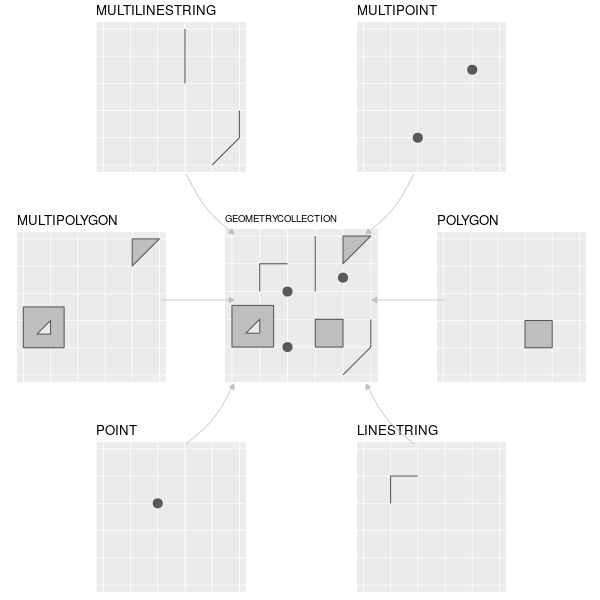
\includegraphics[width=0.65\linewidth,height=\textheight,keepaspectratio]{images/01_geometries.png}
\end{center}
\end{frame}

\begin{frame}{Какие пространственные примитивы можно здесь найти?}
\phantomsection\label{ux43aux430ux43aux438ux435-ux43fux440ux43eux441ux442ux440ux430ux43dux441ux442ux432ux435ux43dux43dux44bux435-ux43fux440ux438ux43cux438ux442ux438ux432ux44b-ux43cux43eux436ux43dux43e-ux437ux434ux435ux441ux44c-ux43dux430ux439ux442ux438}
\begin{center}
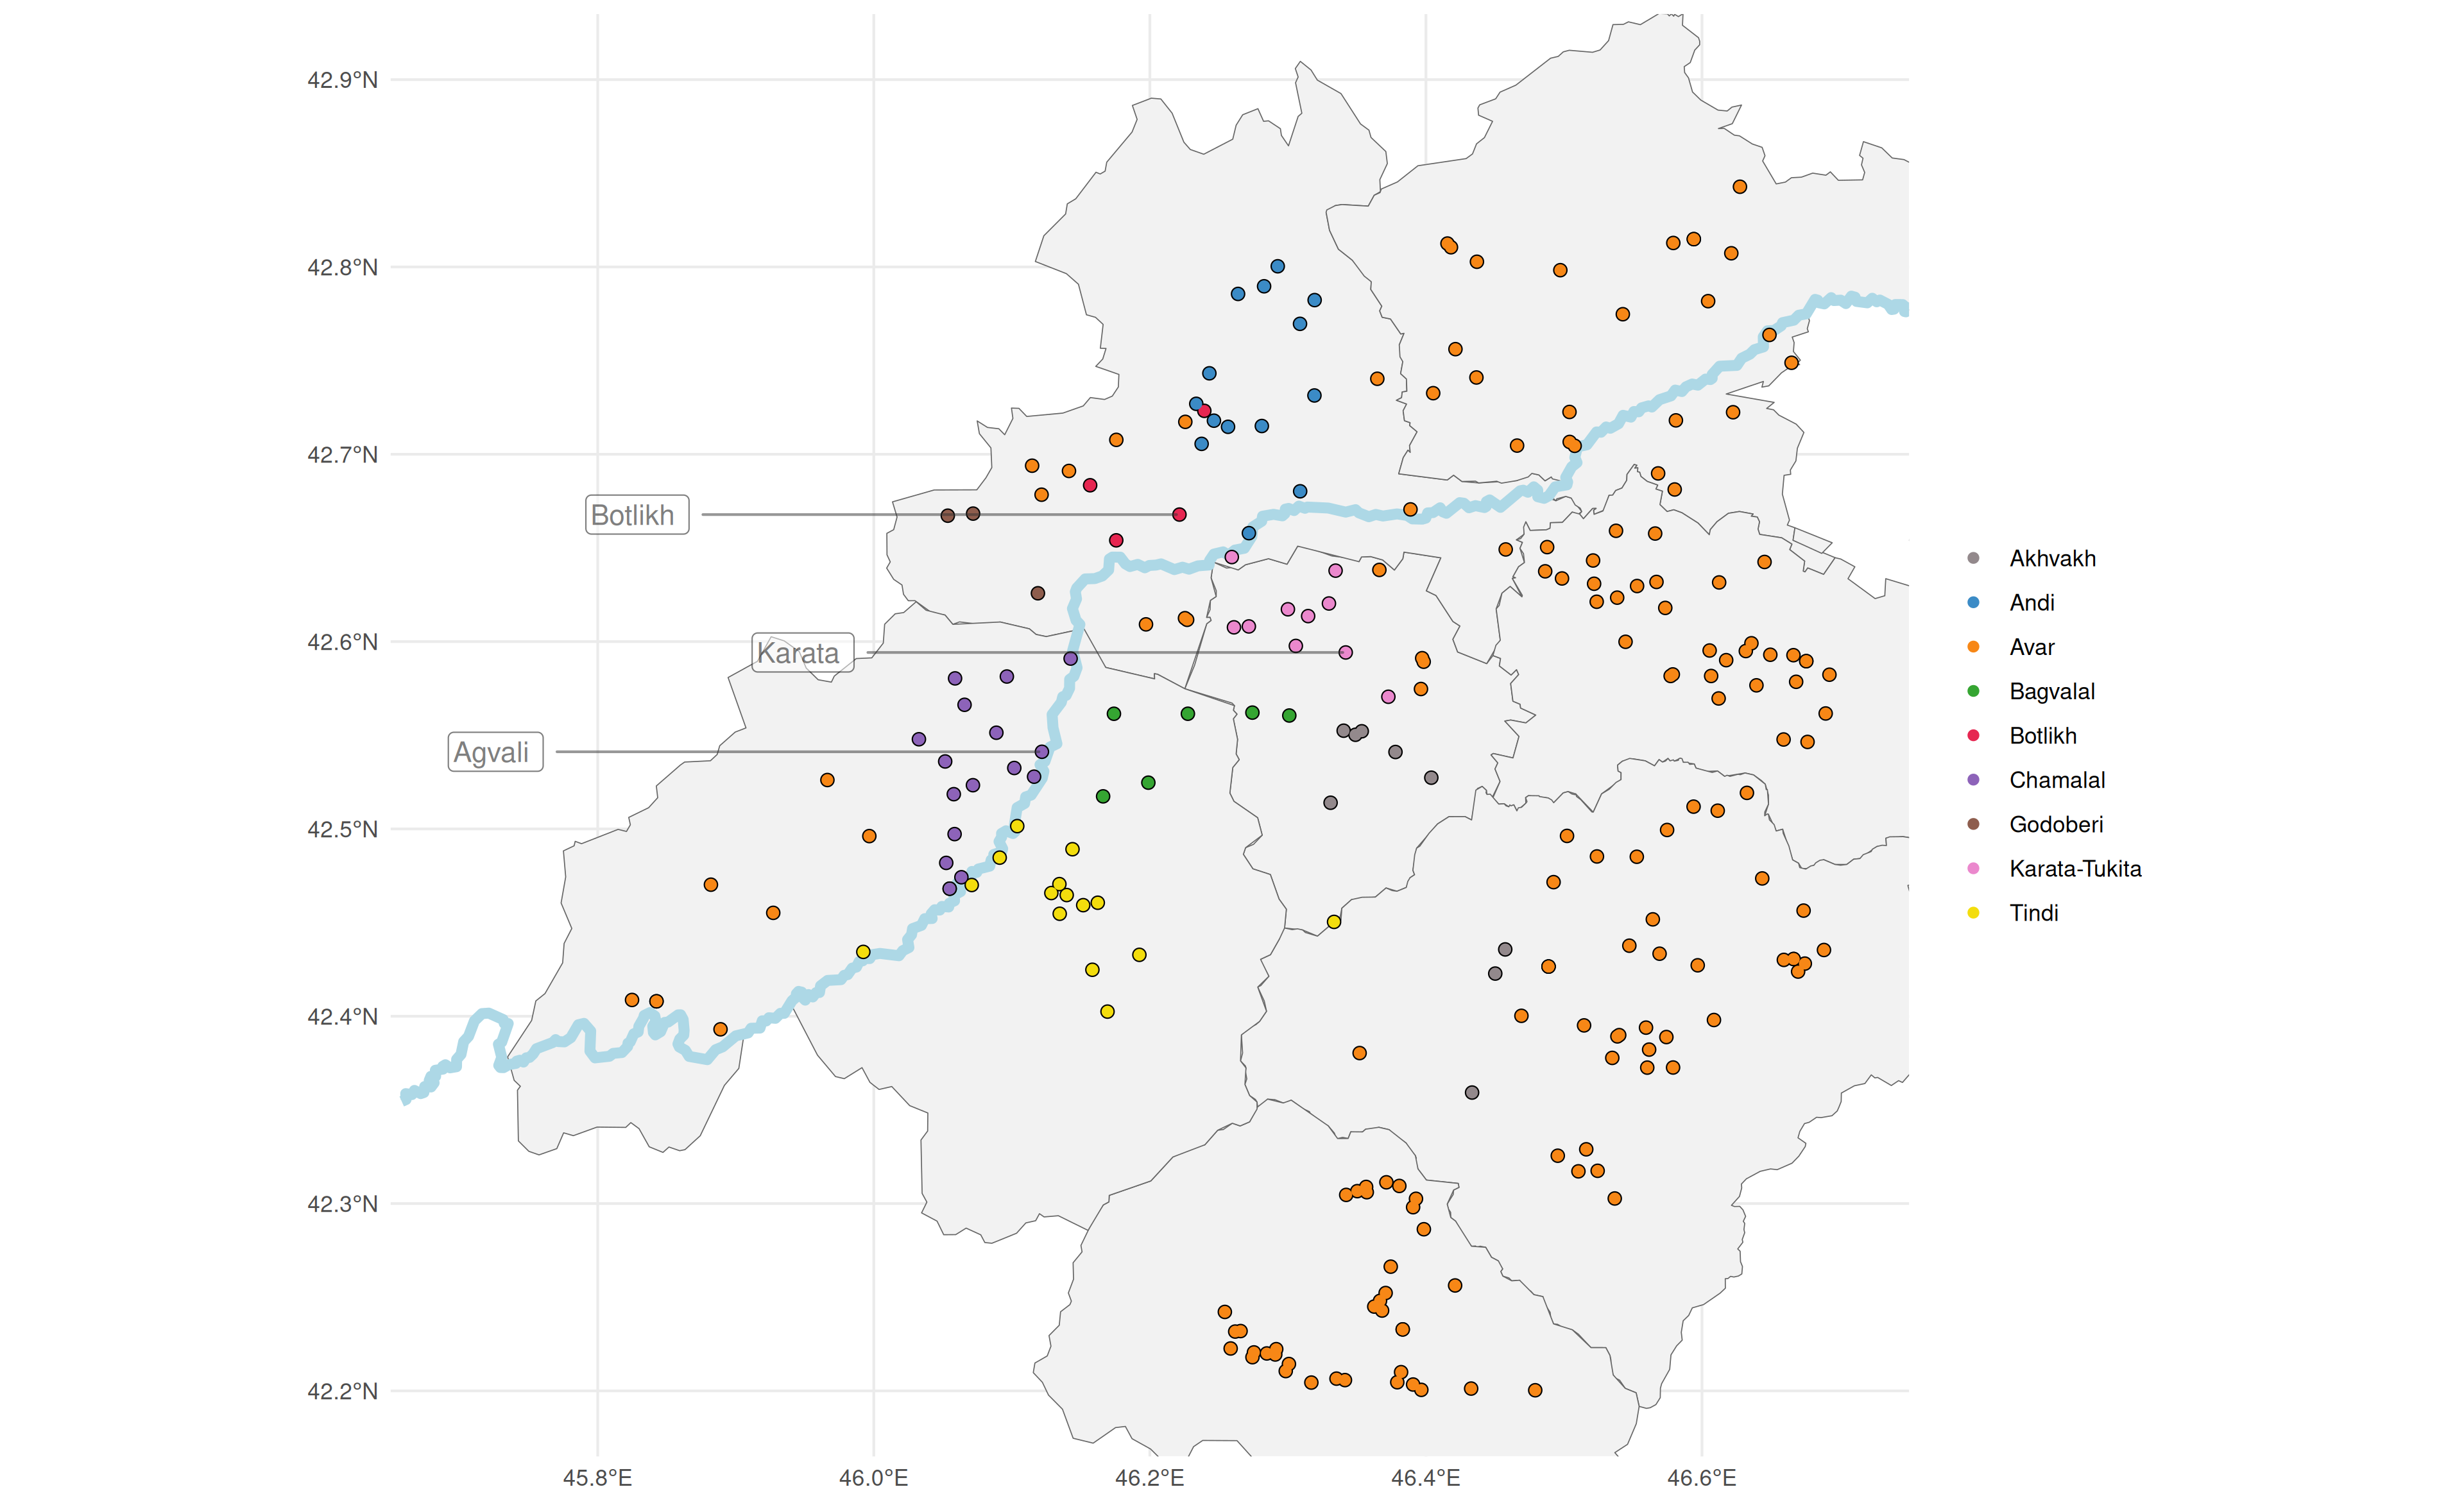
\includegraphics[width=1.15\linewidth,height=\textheight,keepaspectratio]{images/02_dagestan.png}
\end{center}
\end{frame}

\begin{frame}{Чего, как Вам кажется, здесь не хватает?}
\phantomsection\label{ux447ux435ux433ux43e-ux43aux430ux43a-ux432ux430ux43c-ux43aux430ux436ux435ux442ux441ux44f-ux437ux434ux435ux441ux44c-ux43dux435-ux445ux432ux430ux442ux430ux435ux442}
\begin{center}
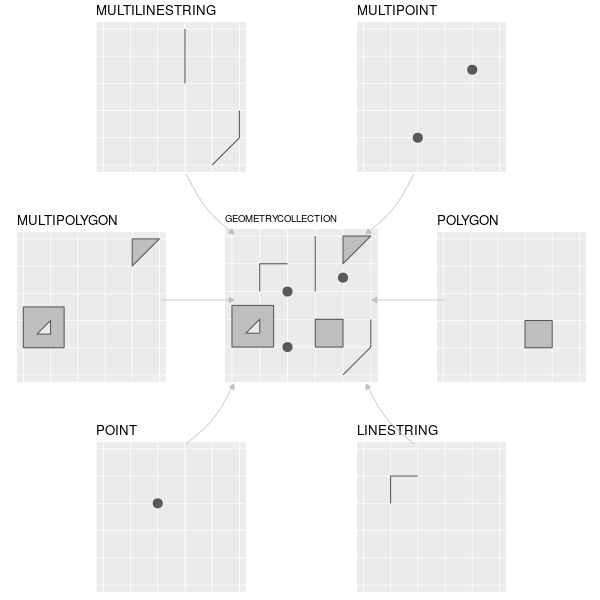
\includegraphics[width=0.65\linewidth,height=\textheight,keepaspectratio]{images/01_geometries.png}
\end{center}

\pause

Мне не хватает объема (т. е. учета высотности).
\end{frame}

\begin{frame}{Растровые данные}
\phantomsection\label{ux440ux430ux441ux442ux440ux43eux432ux44bux435-ux434ux430ux43dux43dux44bux435}
Иногда географические данные не представляют собой не набор
пространственных примитивов.

\begin{itemize}
\tightlist
\item
  сетка некоторой частоты, с некоторым приписанным значением каждой
  ячейке \pause
\item
  растровый объект, например, карта XVI века, которая даже не имеет
  привязки к современной системе координат
\end{itemize}
\end{frame}

\begin{frame}{Кладбище Стародуб (данные полевого архива
\href{https://sfira.org/}{SFIRA})}
\phantomsection\label{ux43aux43bux430ux434ux431ux438ux449ux435-ux441ux442ux430ux440ux43eux434ux443ux431-ux434ux430ux43dux43dux44bux435-ux43fux43eux43bux435ux432ux43eux433ux43e-ux430ux440ux445ux438ux432ux430-sfira}
\pandocbounded{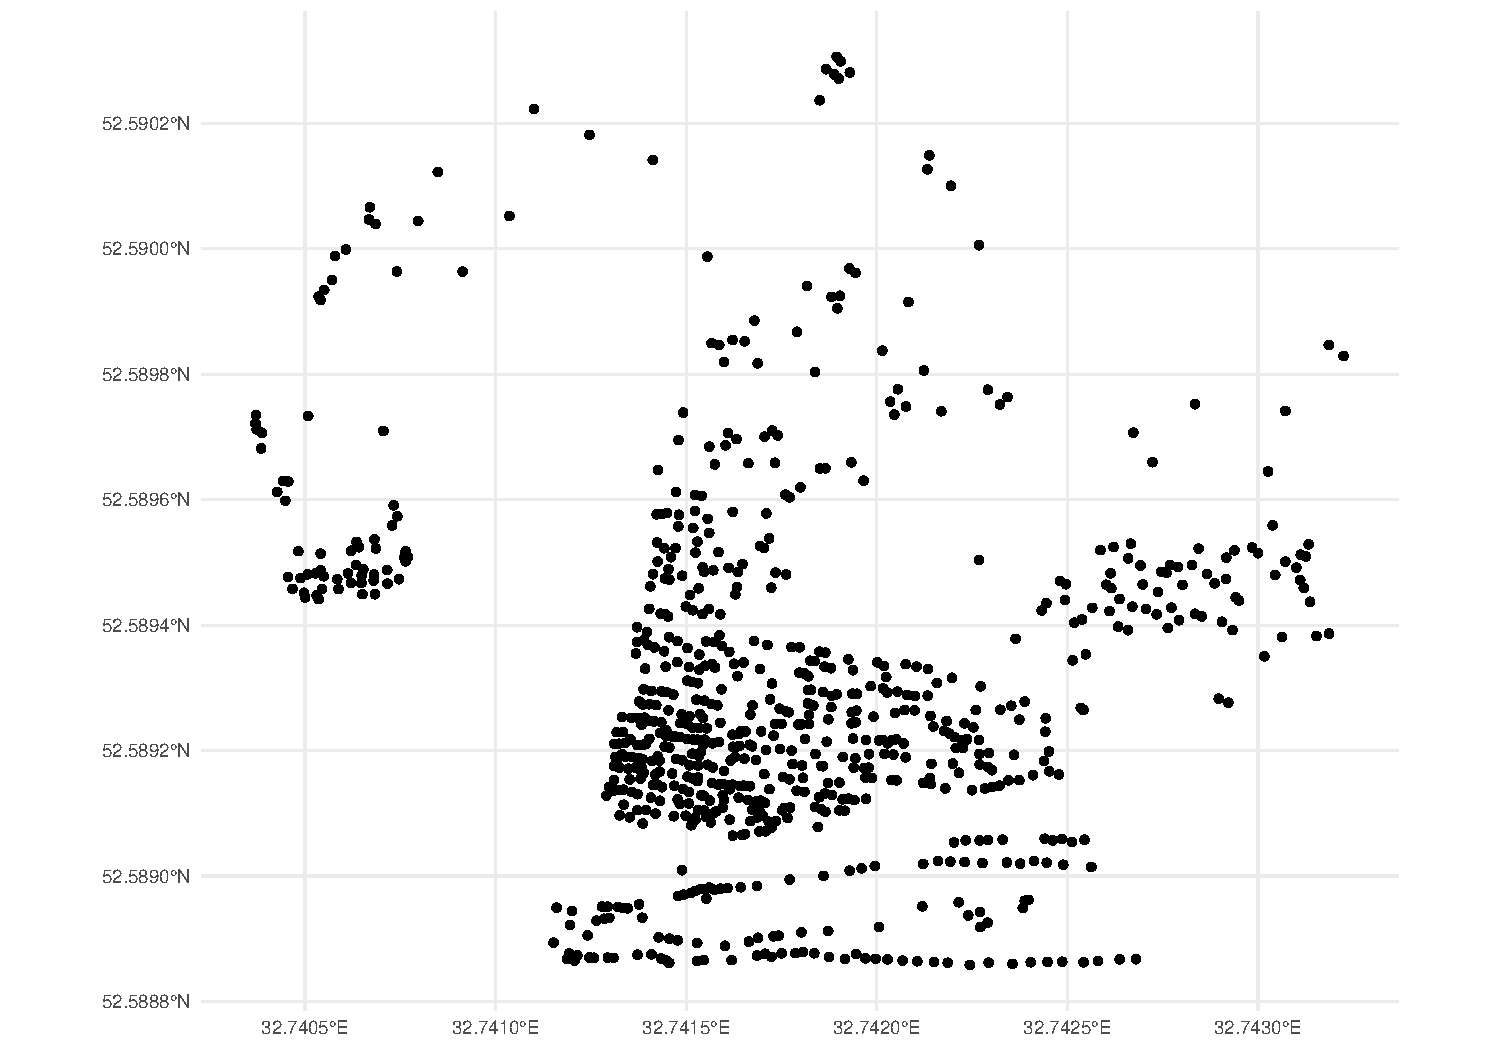
\includegraphics[keepaspectratio]{2025.04.24_HSE_DH_geo_time_files/figure-beamer/unnamed-chunk-5-1.pdf}}
\end{frame}

\begin{frame}{Кладбище Стародуб (данные полевого архива
\href{https://sfira.org/}{SFIRA})}
\phantomsection\label{ux43aux43bux430ux434ux431ux438ux449ux435-ux441ux442ux430ux440ux43eux434ux443ux431-ux434ux430ux43dux43dux44bux435-ux43fux43eux43bux435ux432ux43eux433ux43e-ux430ux440ux445ux438ux432ux430-sfira-1}
\pandocbounded{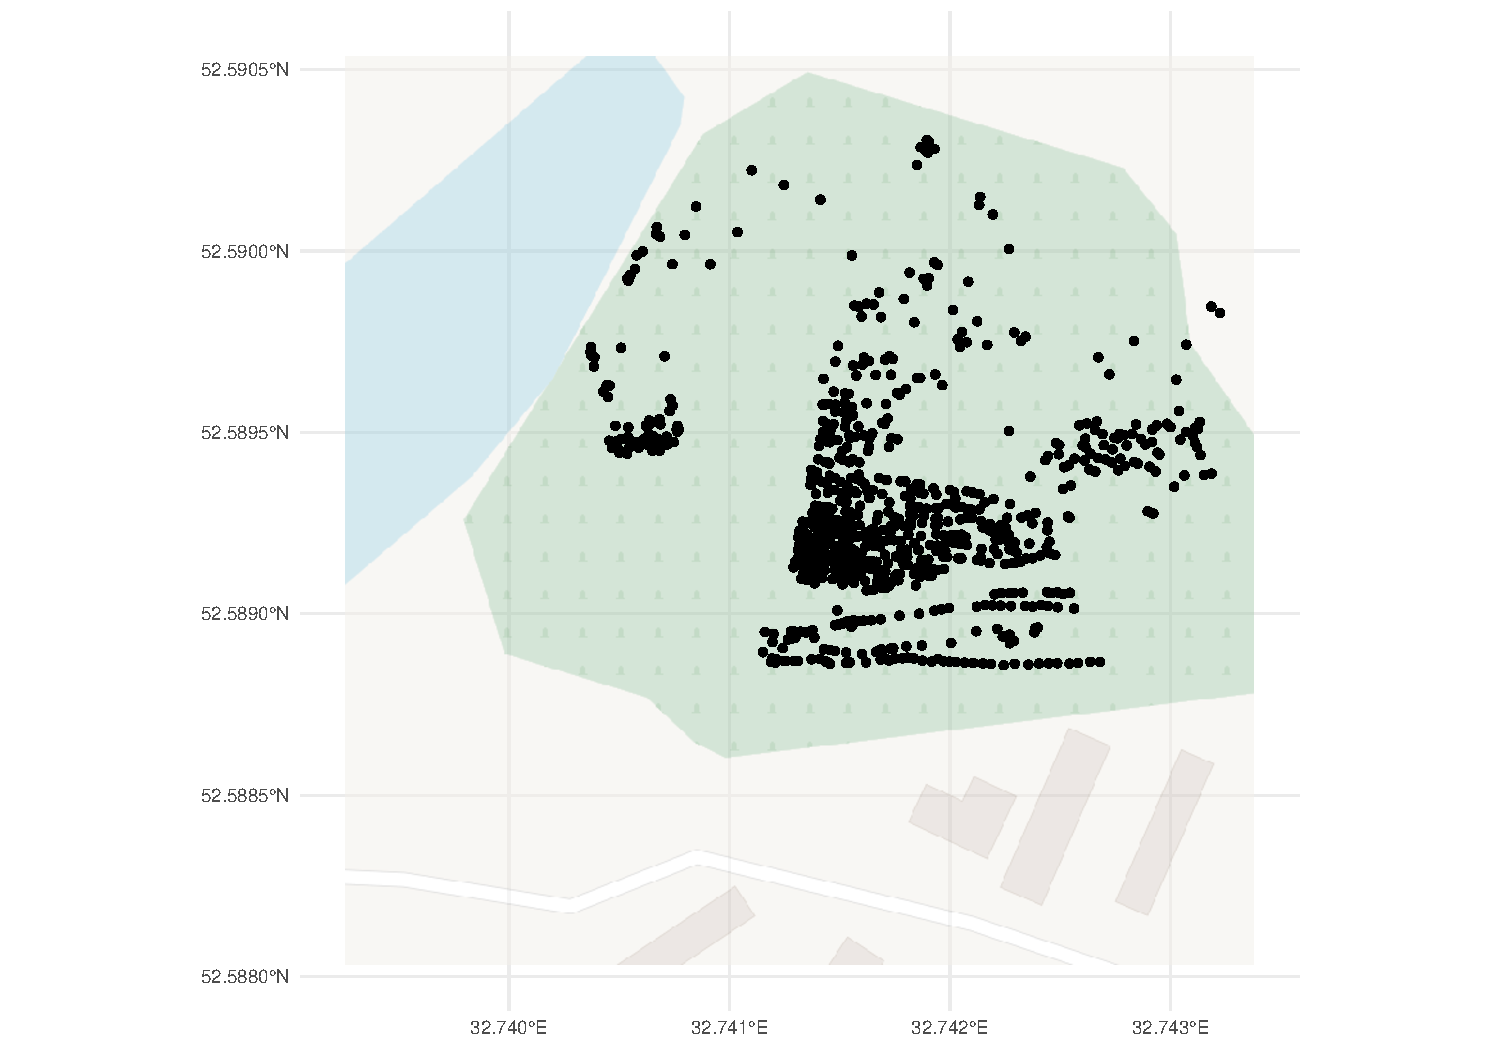
\includegraphics[keepaspectratio]{2025.04.24_HSE_DH_geo_time_files/figure-beamer/unnamed-chunk-6-1.pdf}}
\end{frame}

\begin{frame}{Кладбище Стародуб (данные полевого архива
\href{https://sfira.org/}{SFIRA})}
\phantomsection\label{ux43aux43bux430ux434ux431ux438ux449ux435-ux441ux442ux430ux440ux43eux434ux443ux431-ux434ux430ux43dux43dux44bux435-ux43fux43eux43bux435ux432ux43eux433ux43e-ux430ux440ux445ux438ux432ux430-sfira-2}
\pandocbounded{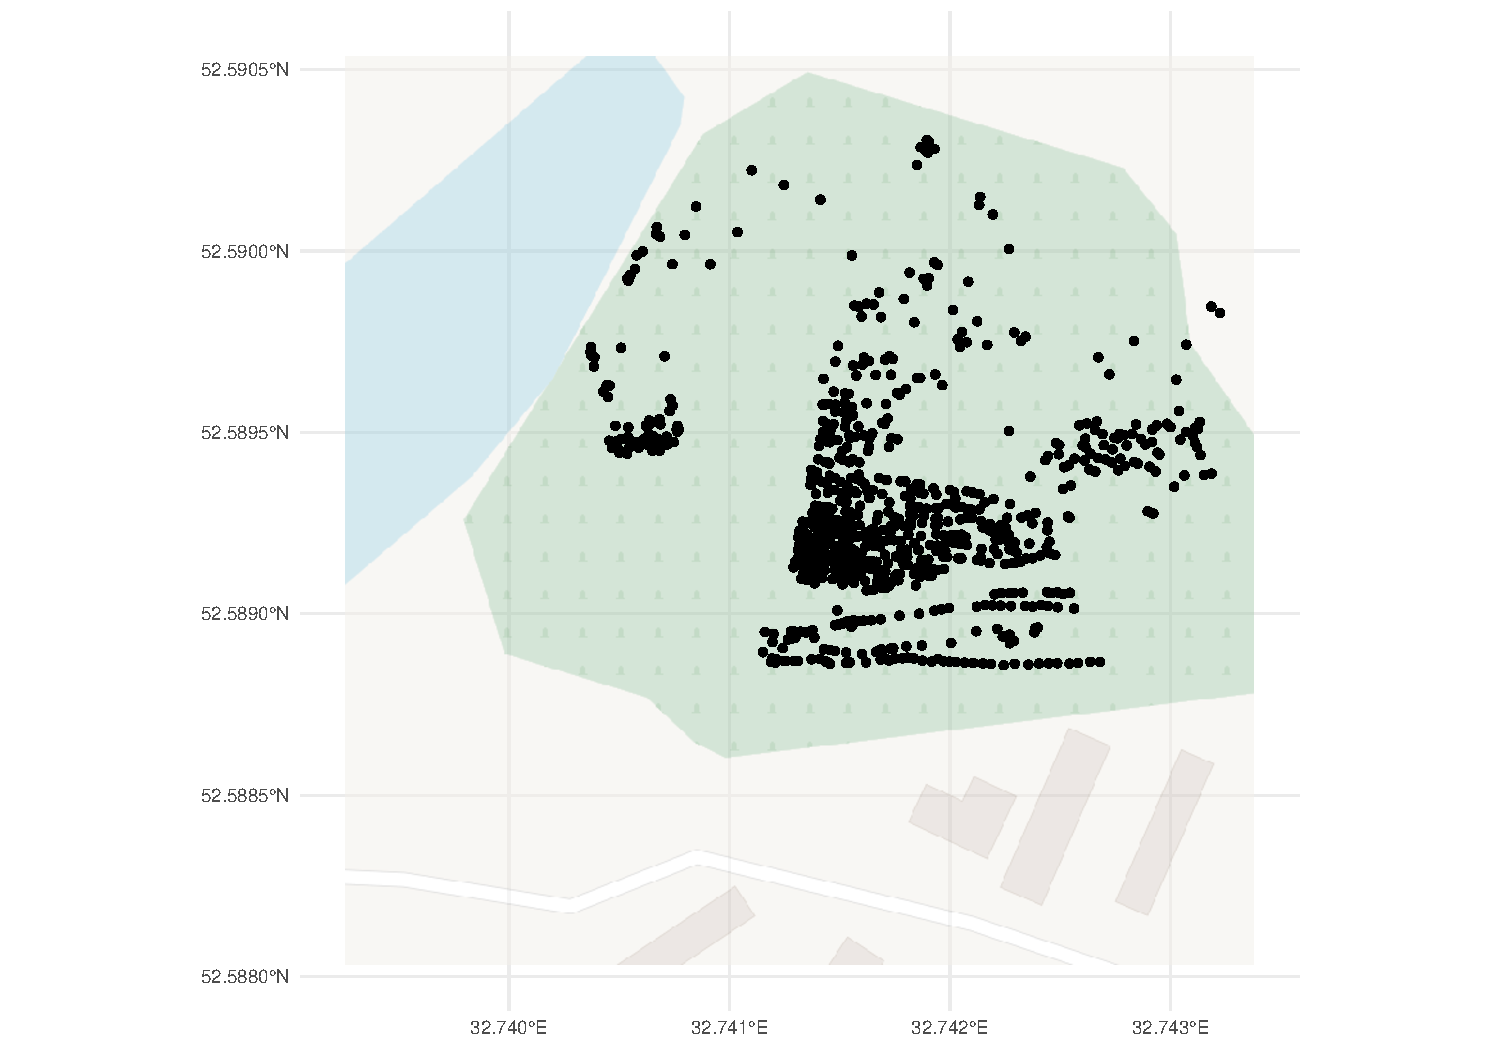
\includegraphics[keepaspectratio]{2025.04.24_HSE_DH_geo_time_files/figure-beamer/unnamed-chunk-7-1.pdf}}
\end{frame}

\begin{frame}{Кладбище Стародуб (данные полевого архива
\href{https://sfira.org/}{SFIRA})}
\phantomsection\label{ux43aux43bux430ux434ux431ux438ux449ux435-ux441ux442ux430ux440ux43eux434ux443ux431-ux434ux430ux43dux43dux44bux435-ux43fux43eux43bux435ux432ux43eux433ux43e-ux430ux440ux445ux438ux432ux430-sfira-3}
\pandocbounded{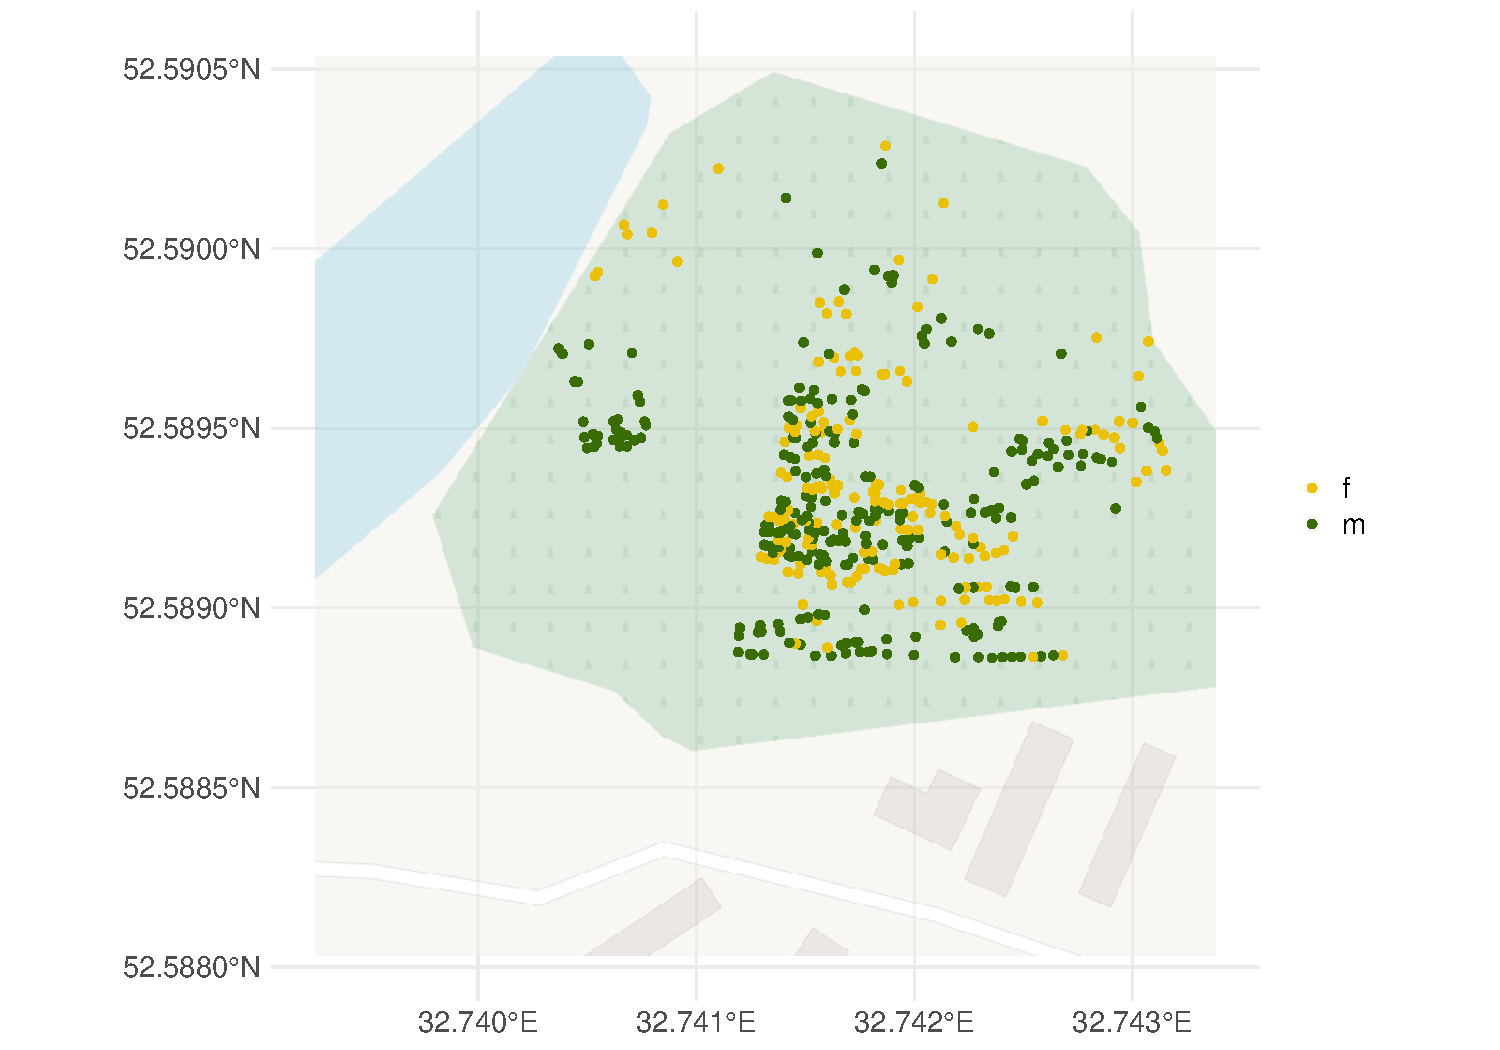
\includegraphics[keepaspectratio]{2025.04.24_HSE_DH_geo_time_files/figure-beamer/unnamed-chunk-8-1.pdf}}
\end{frame}

\begin{frame}{Кладбище Стародуб (данные полевого архива
\href{https://sfira.org/}{SFIRA})}
\phantomsection\label{ux43aux43bux430ux434ux431ux438ux449ux435-ux441ux442ux430ux440ux43eux434ux443ux431-ux434ux430ux43dux43dux44bux435-ux43fux43eux43bux435ux432ux43eux433ux43e-ux430ux440ux445ux438ux432ux430-sfira-4}
\pandocbounded{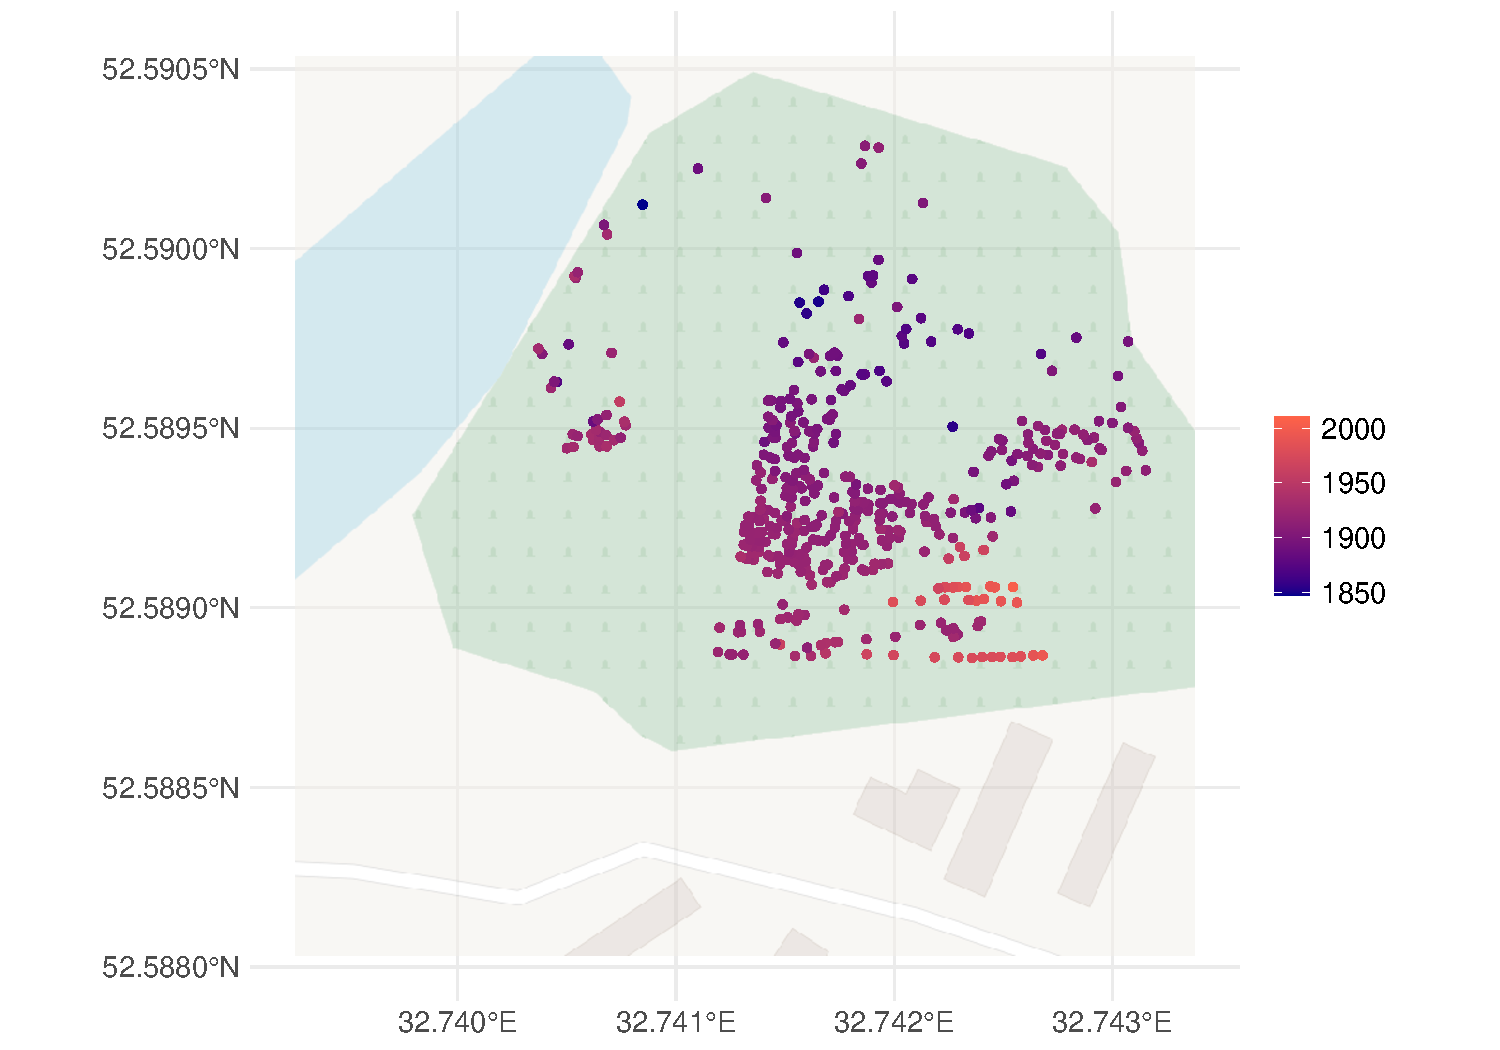
\includegraphics[keepaspectratio]{2025.04.24_HSE_DH_geo_time_files/figure-beamer/unnamed-chunk-9-1.pdf}}
\end{frame}

\begin{frame}{\href{https://agricolamz.github.io/2021.11.10_epigraphy/}{Кладбище
Стародуб} (данные полевого архива \href{https://sfira.org/}{SFIRA})}
\phantomsection\label{ux43aux43bux430ux434ux431ux438ux449ux435-ux441ux442ux430ux440ux43eux434ux443ux431-ux434ux430ux43dux43dux44bux435-ux43fux43eux43bux435ux432ux43eux433ux43e-ux430ux440ux445ux438ux432ux430-sfira-5}
\pandocbounded{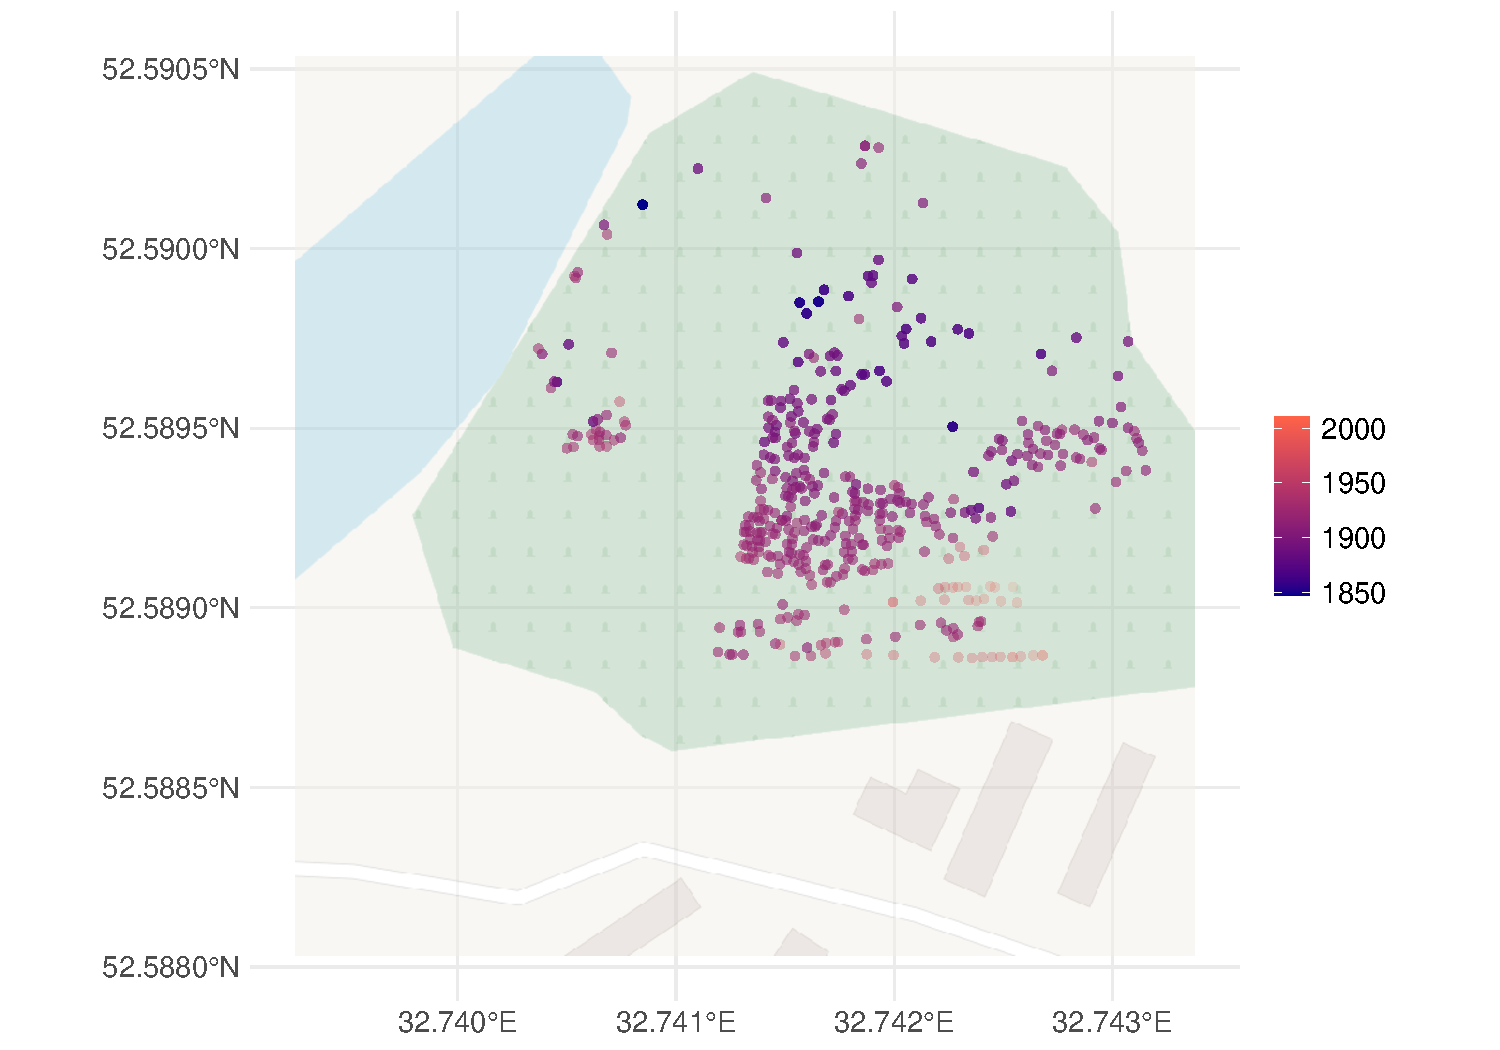
\includegraphics[keepaspectratio]{2025.04.24_HSE_DH_geo_time_files/figure-beamer/unnamed-chunk-10-1.pdf}}
\end{frame}

\begin{frame}{Ошибка выжевшего: Абрахам Вальд}
\phantomsection\label{ux43eux448ux438ux431ux43aux430-ux432ux44bux436ux435ux432ux448ux435ux433ux43e-ux430ux431ux440ux430ux445ux430ux43c-ux432ux430ux43bux44cux434}
\begin{center}
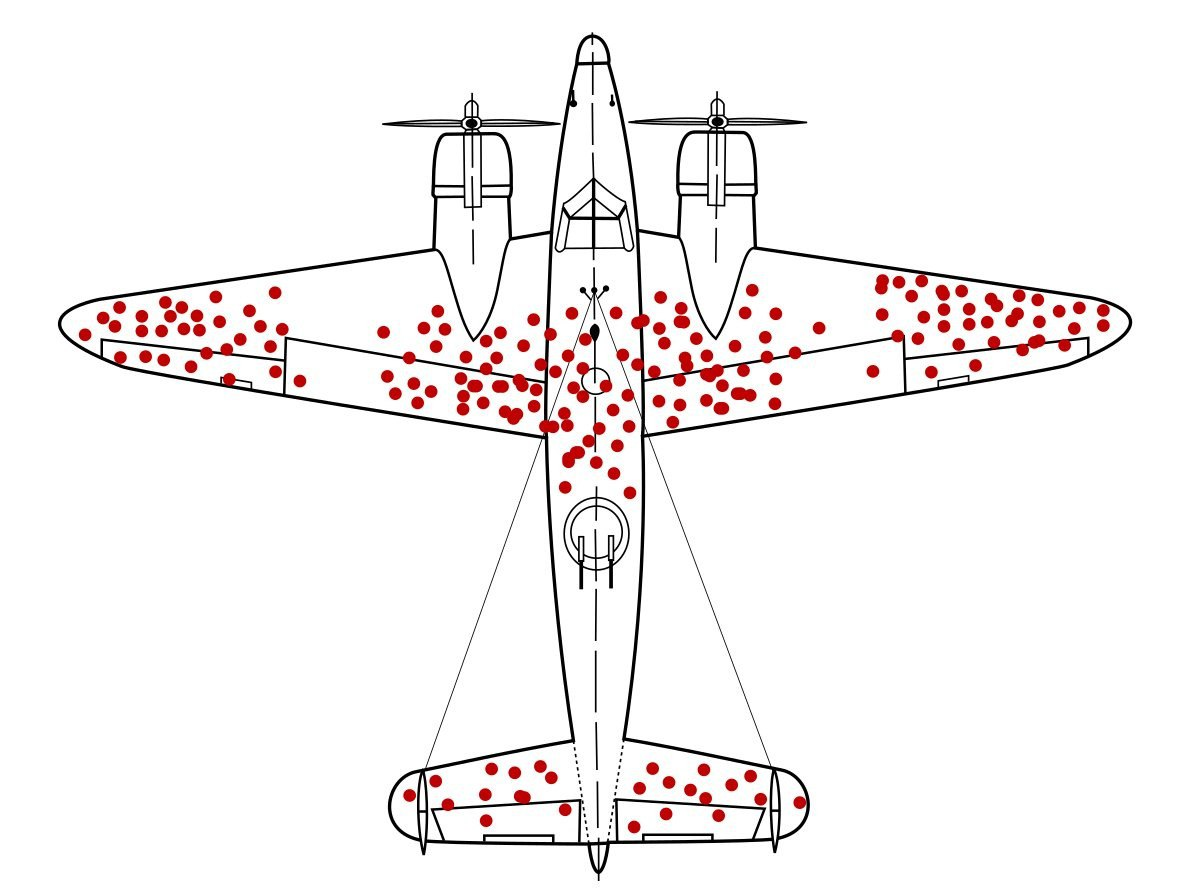
\includegraphics[width=1\linewidth,height=\textheight,keepaspectratio]{images/03_airplane.jpg}
\end{center}
\end{frame}

\begin{frame}{Картографическая проекция}
\phantomsection\label{ux43aux430ux440ux442ux43eux433ux440ux430ux444ux438ux447ux435ux441ux43aux430ux44f-ux43fux440ux43eux435ux43aux446ux438ux44f}
Любое отображение некоторого небесного тела на плоскость называют
картографической проекцией.

Если расстояния в ваших данных небольшие (особенно, если координаты
близки к экватору), широту и долготу можно без страха использовать как
оси в декартовой системе координат (она же --- проекция Меркатора).
Однако при работе с данными масштаба страны/континента/планеты такой
подход будет накопливать ошибку из-за искажений одного из следующих
типов:

\begin{itemize}
\tightlist
\item
  искажения длин;
\item
  искажения углов;
\item
  искажения площадей;
\item
  искажения форм.
\end{itemize}
\end{frame}

\begin{frame}{Картографическая проекция}
\phantomsection\label{ux43aux430ux440ux442ux43eux433ux440ux430ux444ux438ux447ux435ux441ux43aux430ux44f-ux43fux440ux43eux435ux43aux446ux438ux44f-1}
Проекция Меркатора очень сильно искажает площади:

\begin{figure}

\begin{minipage}{0.50\linewidth}

\begin{figure}[H]

{\centering 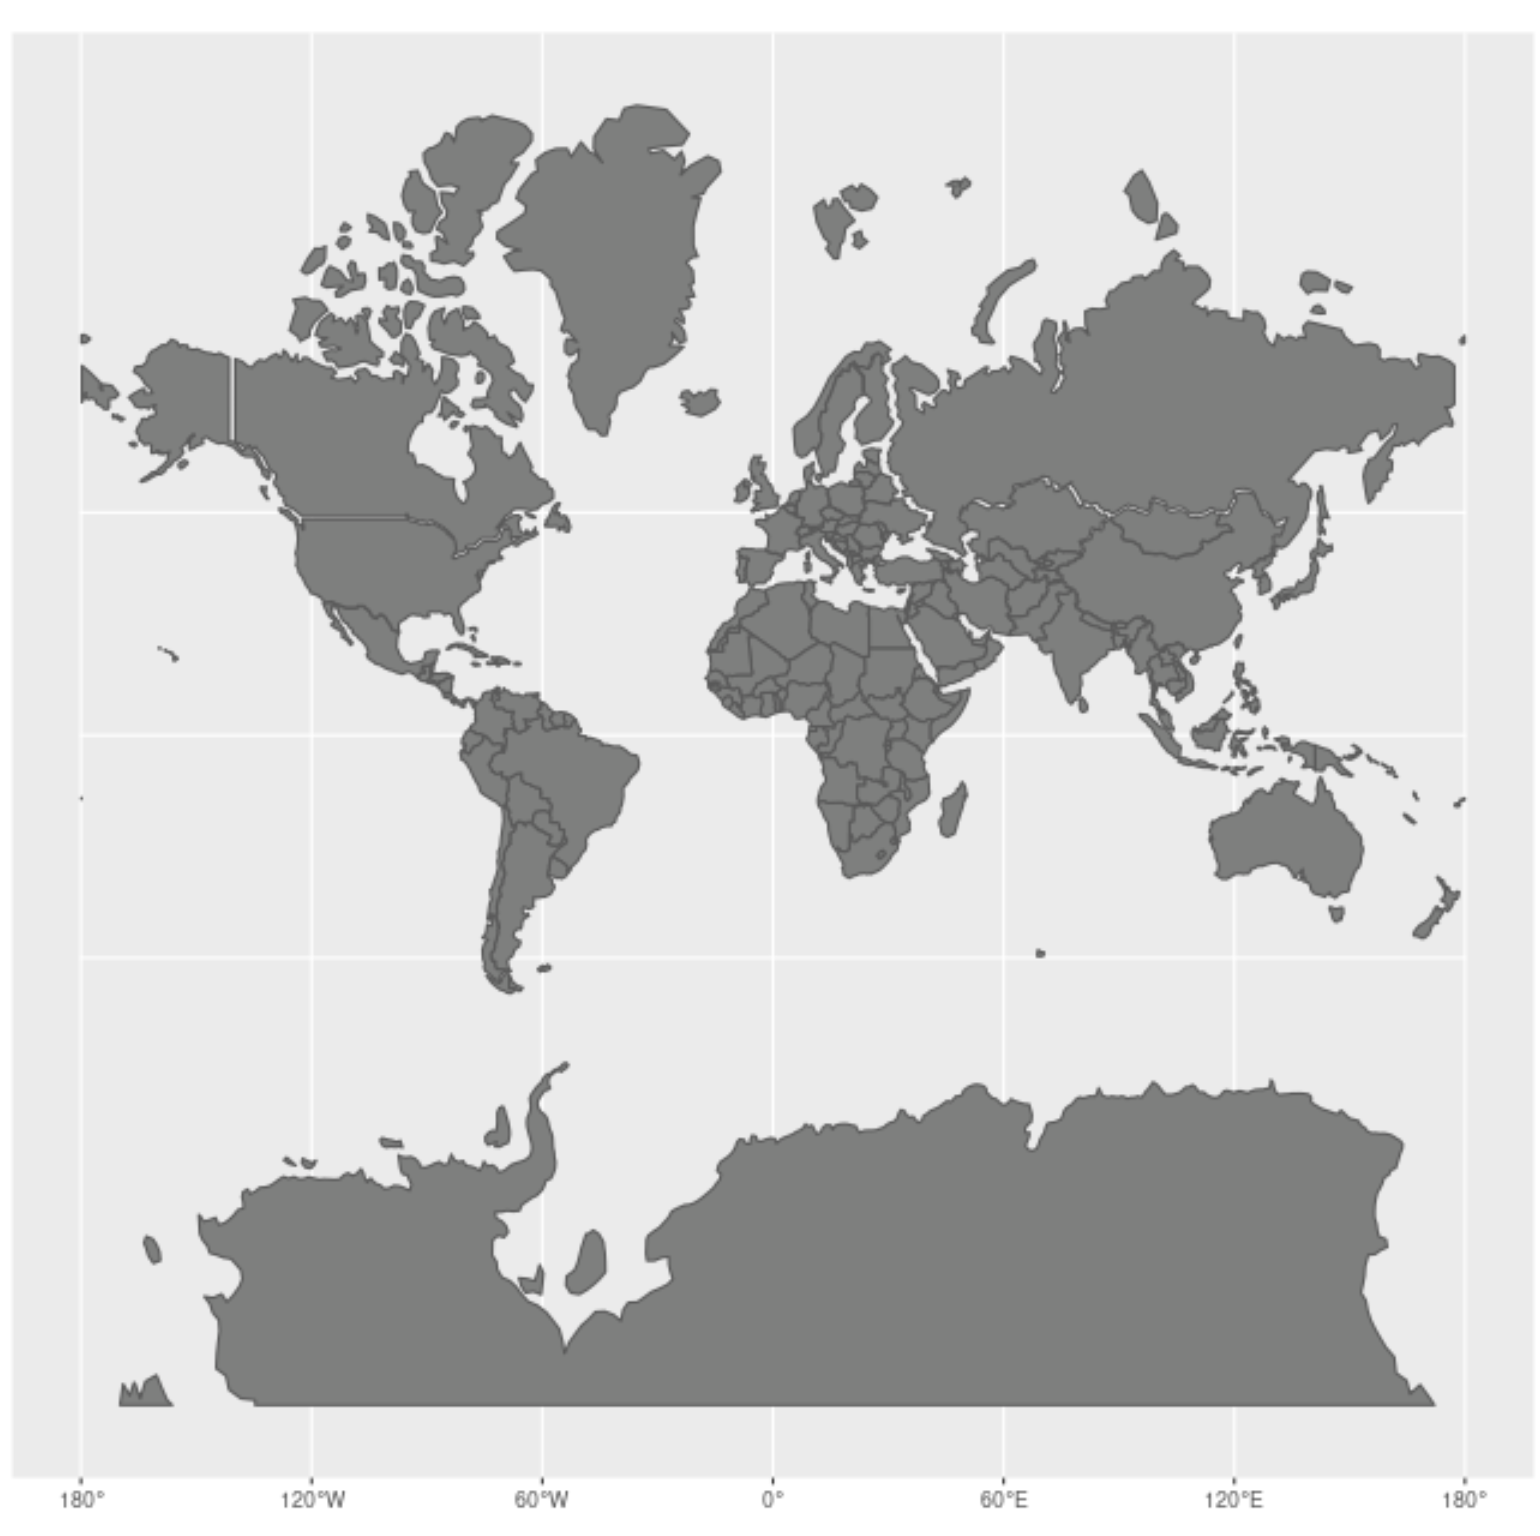
\includegraphics[width=1\linewidth,height=\textheight,keepaspectratio]{images/07-Merkator-1.png}

}

\subcaption{исходный}

\end{figure}%

\end{minipage}%
%
\begin{minipage}{0.50\linewidth}

\begin{figure}[H]

{\centering 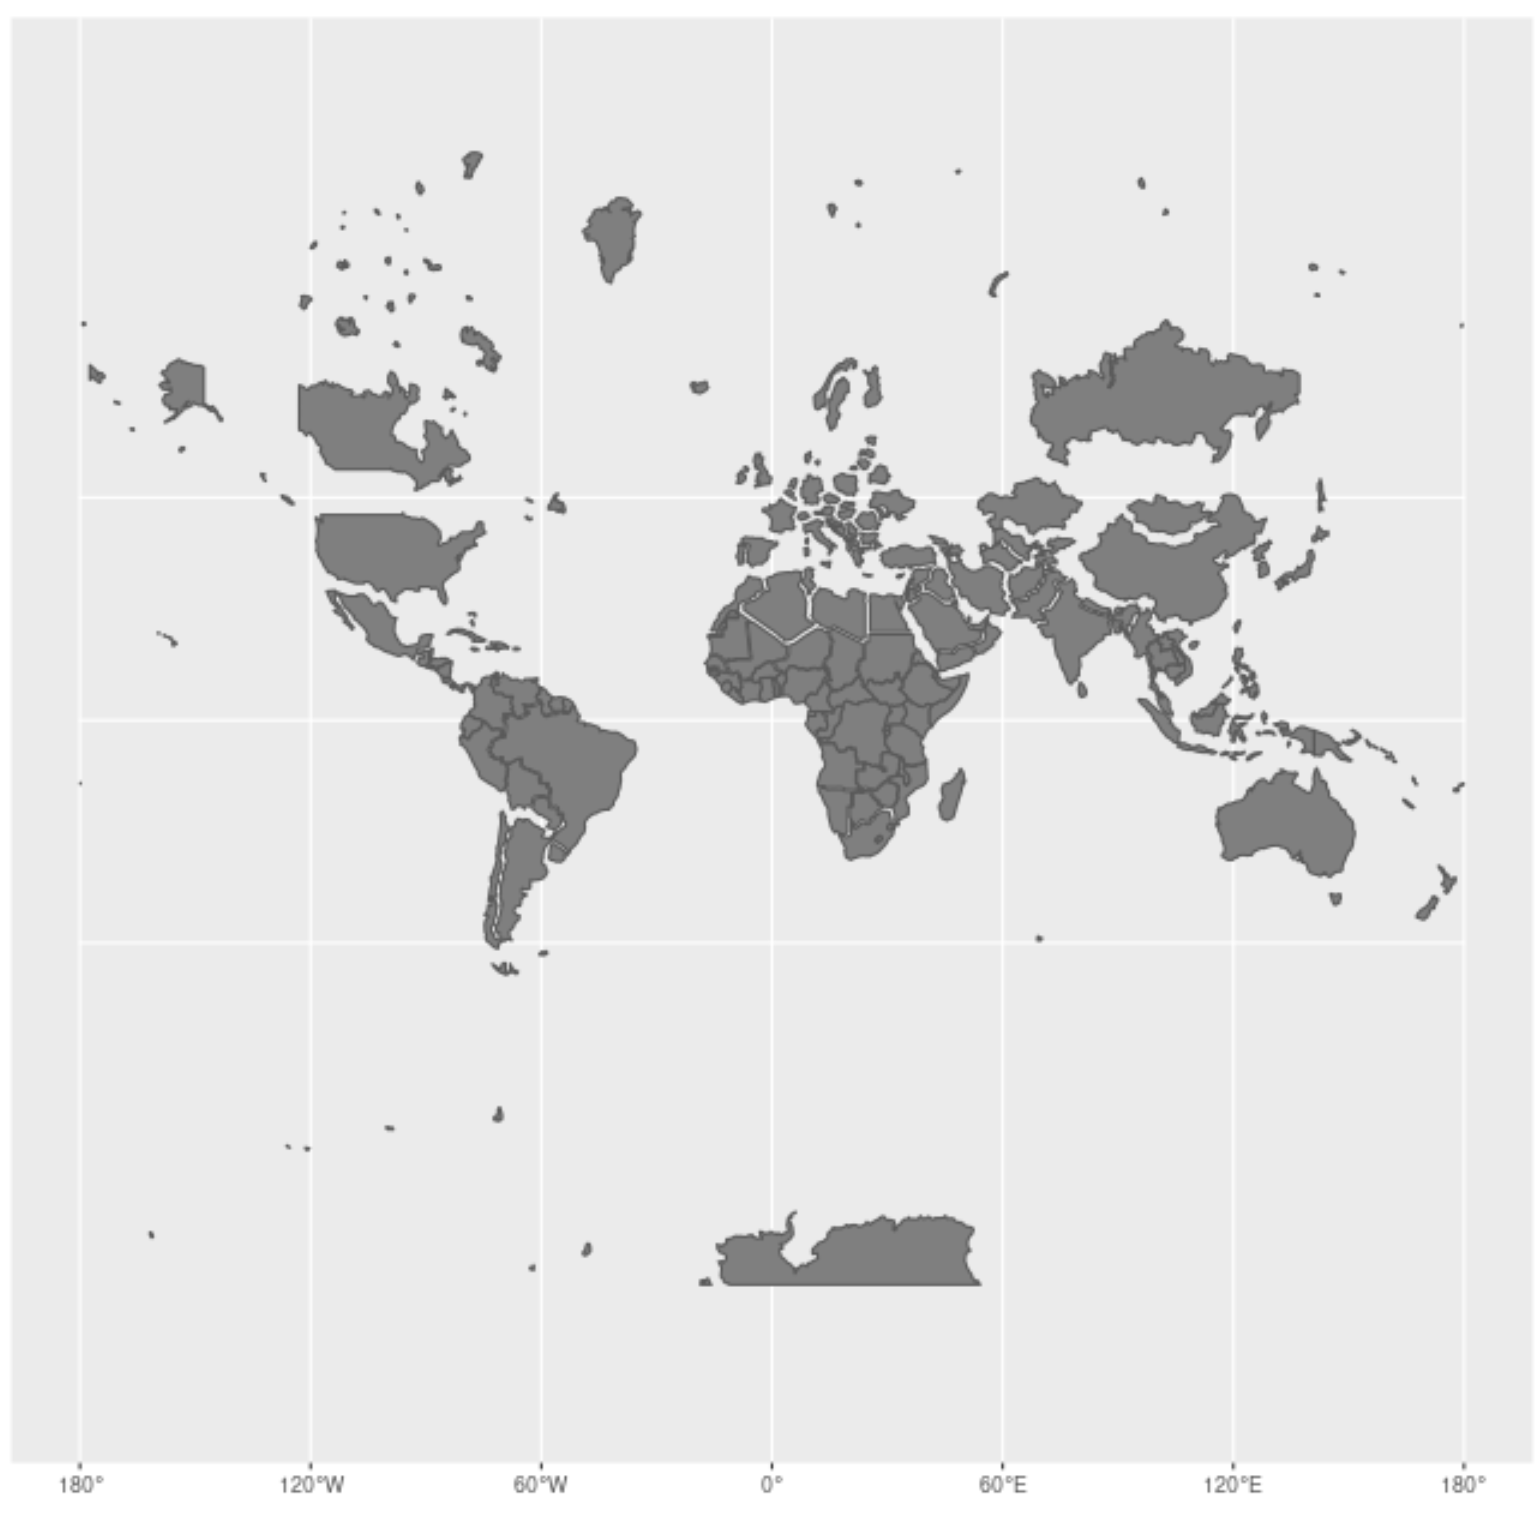
\includegraphics[width=1\linewidth,height=\textheight,keepaspectratio]{images/08-Merkator-2.png}

}

\subcaption{с сохранением площадей}

\end{figure}%

\end{minipage}%
\newline
\begin{minipage}{0.50\linewidth}
источник --- Википедия\end{minipage}%

\end{figure}%
\end{frame}

\begin{frame}{Картографическая проекция}
\phantomsection\label{ux43aux430ux440ux442ux43eux433ux440ux430ux444ux438ux447ux435ux441ux43aux430ux44f-ux43fux440ux43eux435ux43aux446ux438ux44f-2}
\begin{itemize}
\tightlist
\item
  \href{https://projectionwizard.org/}{веб-приложение}, помогающее
  выбрать подходящую проекцию
\item
  \href{https://mathigon.org/course/circles/spheres-cones-cylinders\#sphere-maps}{веб-приложение},
  которое показывает как изменяются объекты при преобразовании с сферы
  на одну из четырех проекций (Меркатора, цилиндрическую, Робинсона,
  Моллвейде)
\item
  \href{https://proj.org/en/latest/operations/projections/all_images.html}{Здесь}
  содержится список всех возможных проекций
\end{itemize}
\end{frame}

\begin{frame}{Моделирование пространственных отношений}
\phantomsection\label{ux43cux43eux434ux435ux43bux438ux440ux43eux432ux430ux43dux438ux435-ux43fux440ux43eux441ux442ux440ux430ux43dux441ux442ux432ux435ux43dux43dux44bux445-ux43eux442ux43dux43eux448ux435ux43dux438ux439}
Моделирование пространственных отношений позволяет отвечать на вопросы:

\begin{itemize}
\tightlist
\item
  Существует ли какая-то группировка значений исследуемой переменной в
  пространстве?
\item
  Правда ли, что сходные значения имеют тенденцию находиться рядом?
\item
  Можно ли выделить какие-то регионы концентрации каких-то из значений?
\end{itemize}

Однако для ответа на все эти вопросы мы прежде всего должны построить
граф соседства.
\end{frame}

\begin{frame}{Языковое сходство рутульских идиомов}
\phantomsection\label{ux44fux437ux44bux43aux43eux432ux43eux435-ux441ux445ux43eux434ux441ux442ux432ux43e-ux440ux443ux442ux443ux43bux44cux441ux43aux438ux445-ux438ux434ux438ux43eux43cux43eux432}
\pandocbounded{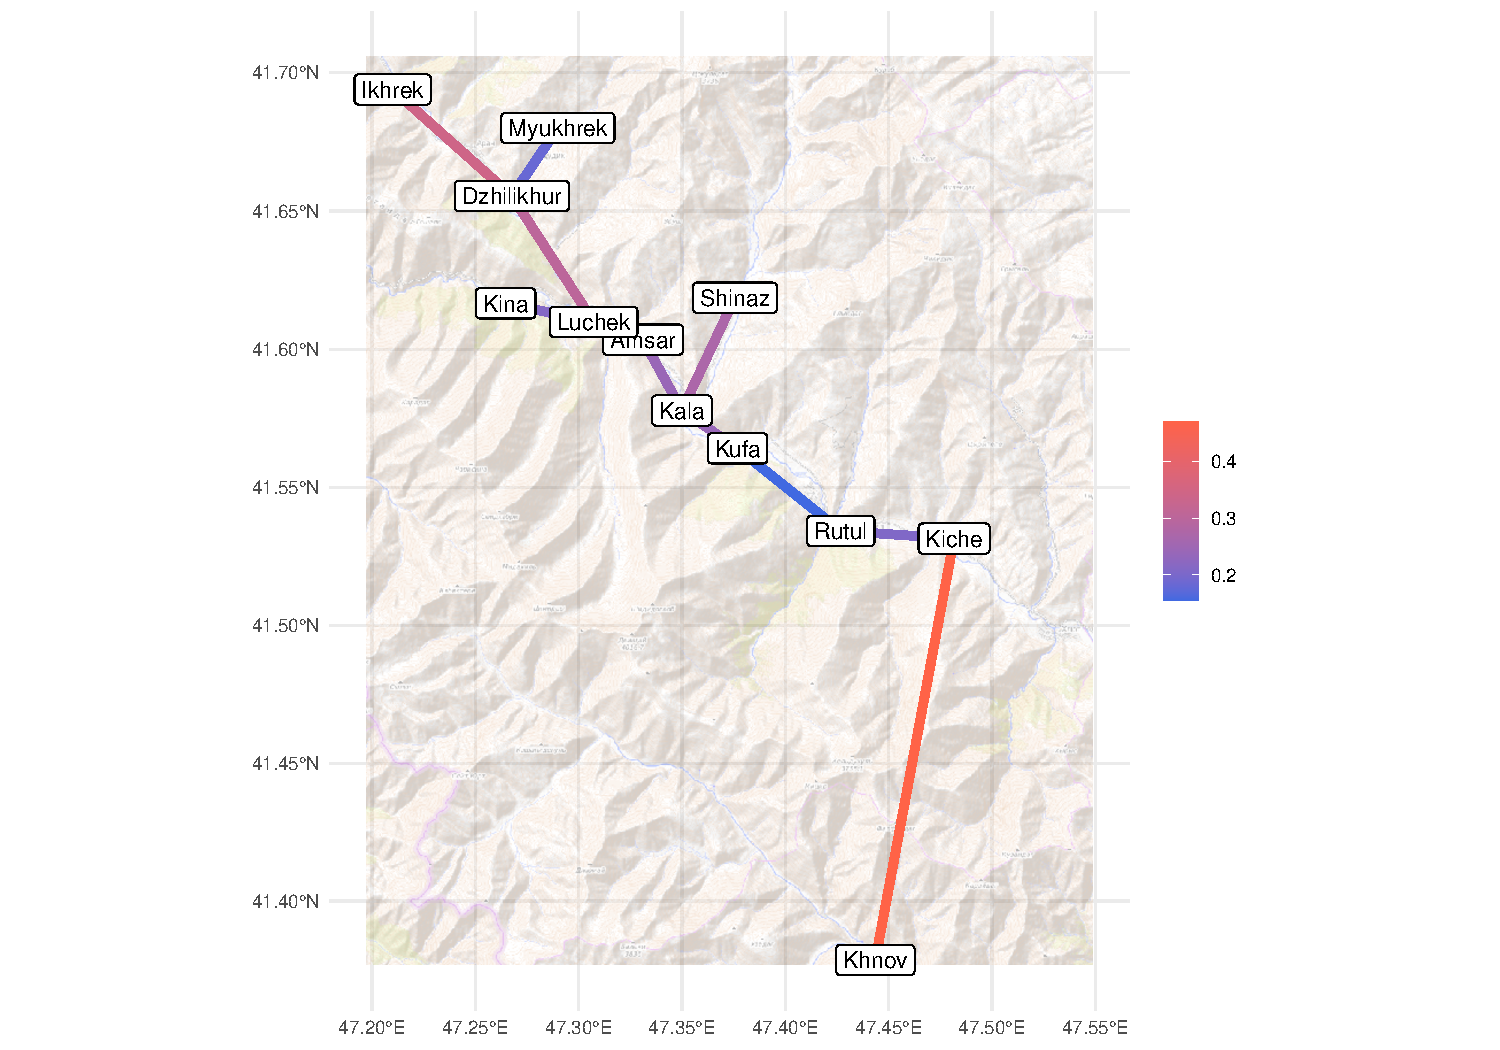
\includegraphics[keepaspectratio]{2025.04.24_HSE_DH_geo_time_files/figure-beamer/unnamed-chunk-13-1.pdf}}
\end{frame}

\begin{frame}{Как определить соседей?}
\phantomsection\label{ux43aux430ux43a-ux43eux43fux440ux435ux434ux435ux43bux438ux442ux44c-ux441ux43eux441ux435ux434ux435ux439}
\begin{center}
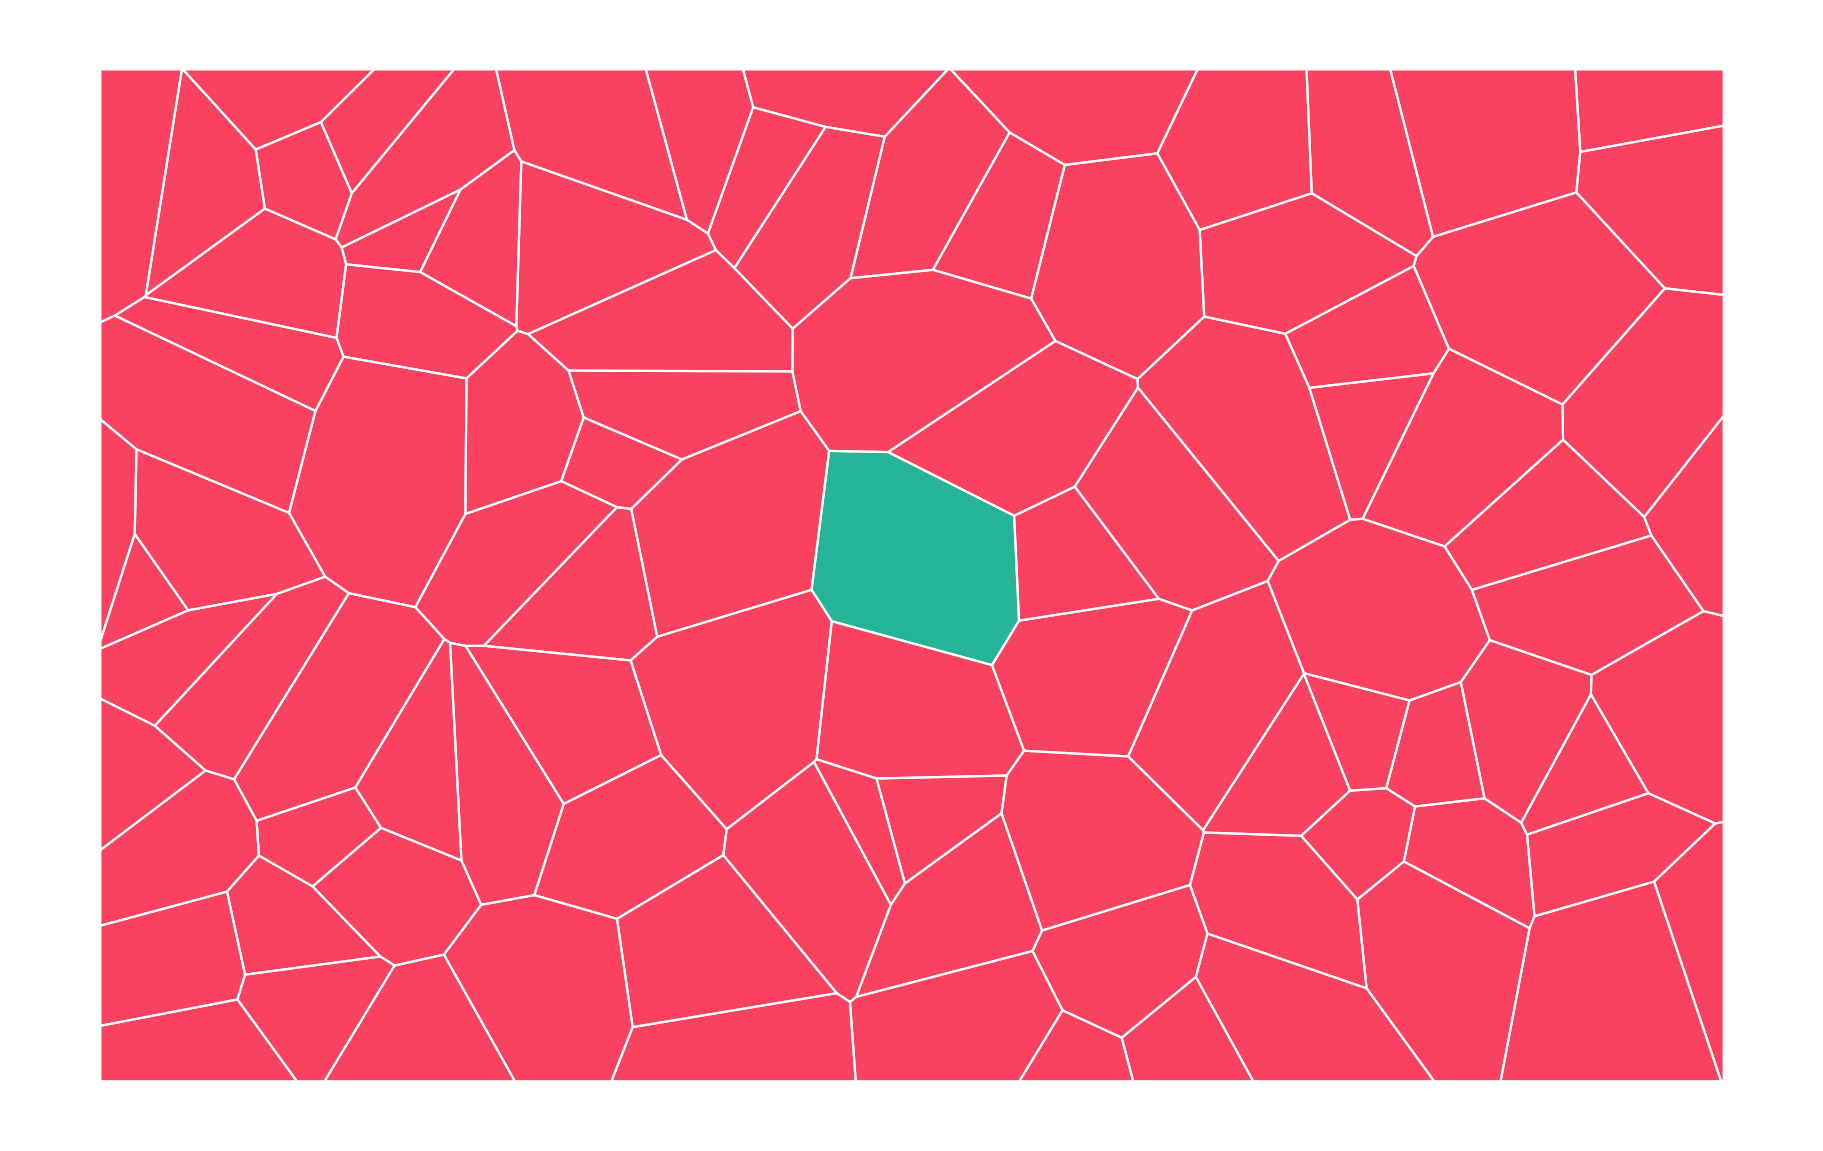
\includegraphics[width=1\linewidth,height=\textheight,keepaspectratio]{images/04-neighbour.png}
\end{center}

Из курса М. Фляйшманна ``Spatial Data Science for Social Geography''
\end{frame}

\begin{frame}{Как определить соседей?}
\phantomsection\label{ux43aux430ux43a-ux43eux43fux440ux435ux434ux435ux43bux438ux442ux44c-ux441ux43eux441ux435ux434ux435ux439-1}
\begin{center}
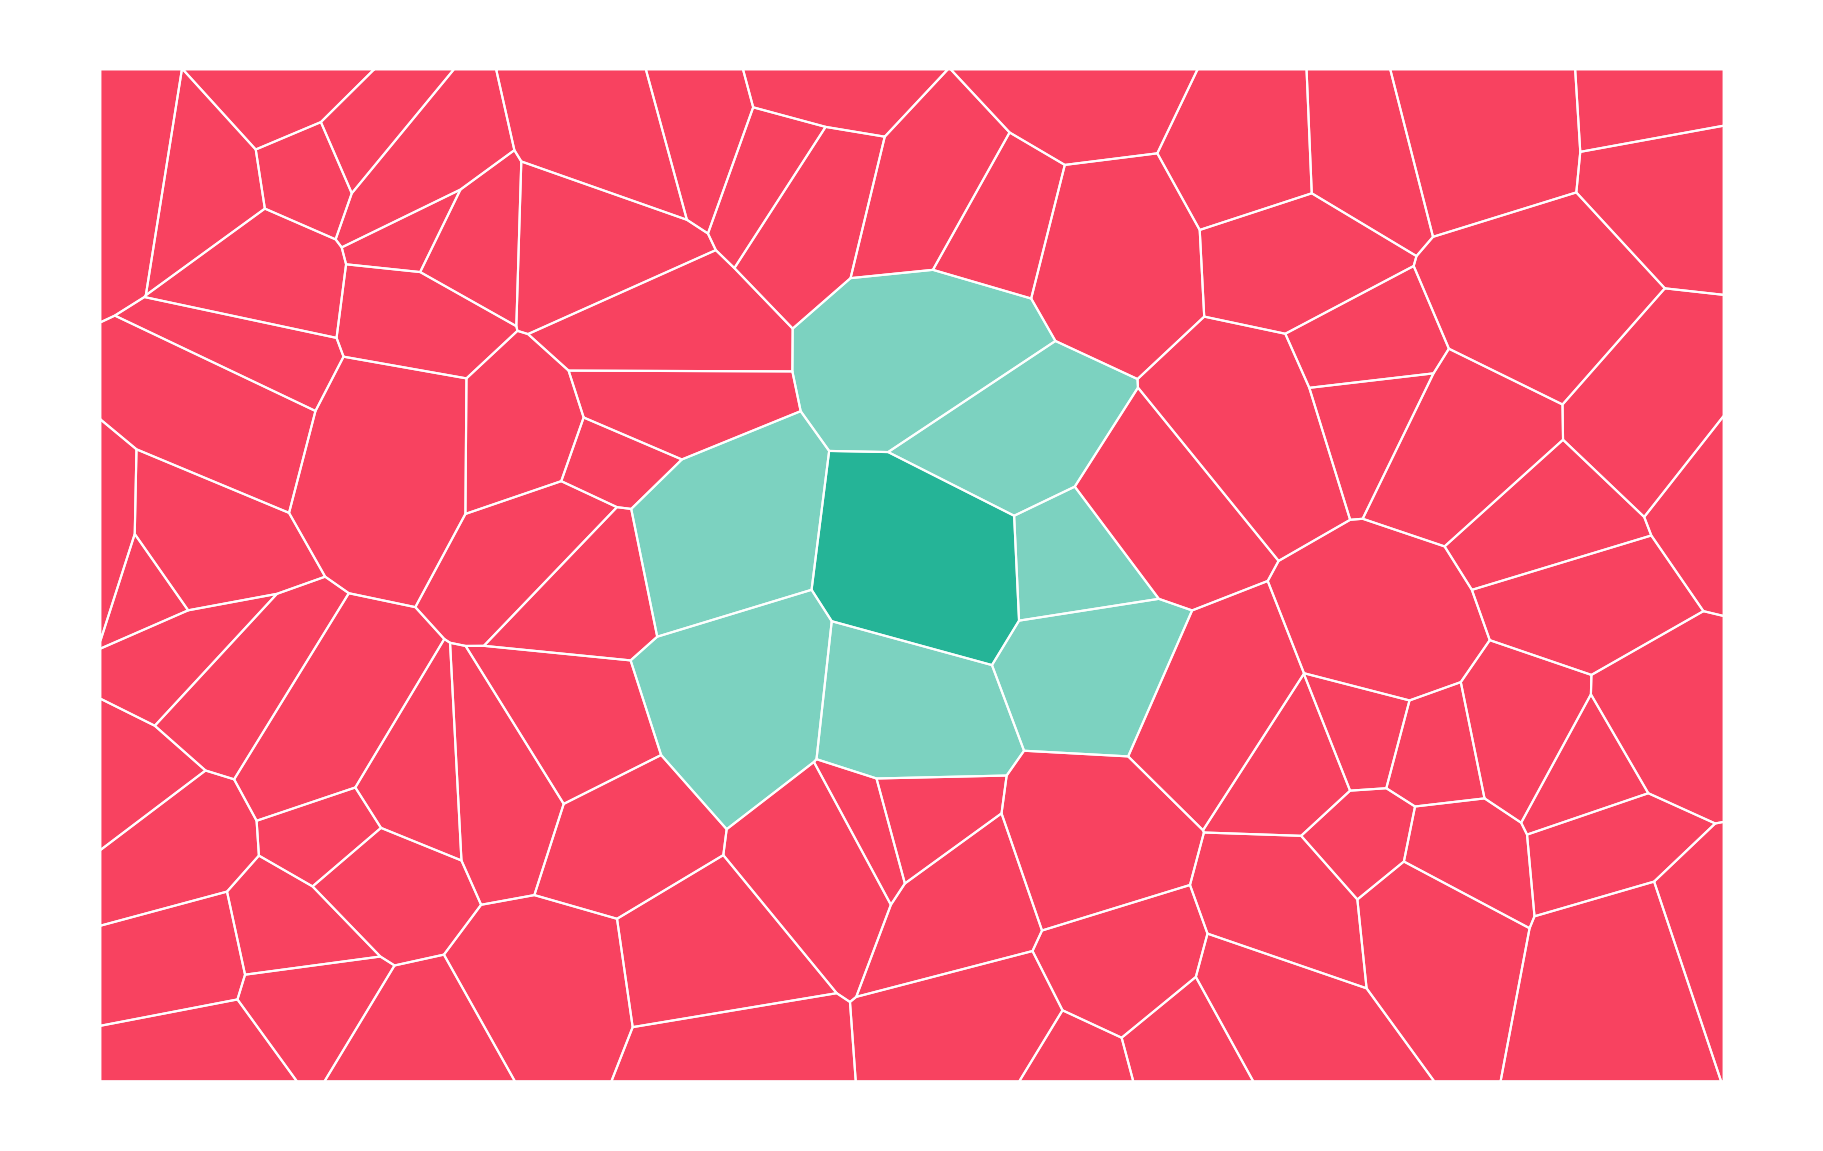
\includegraphics[width=1\linewidth,height=\textheight,keepaspectratio]{images/05-neighbour.png}
\end{center}

Из курса М. Фляйшманна ``Spatial Data Science for Social Geography''
\end{frame}

\begin{frame}{Как определить соседей?}
\phantomsection\label{ux43aux430ux43a-ux43eux43fux440ux435ux434ux435ux43bux438ux442ux44c-ux441ux43eux441ux435ux434ux435ux439-2}
\begin{center}
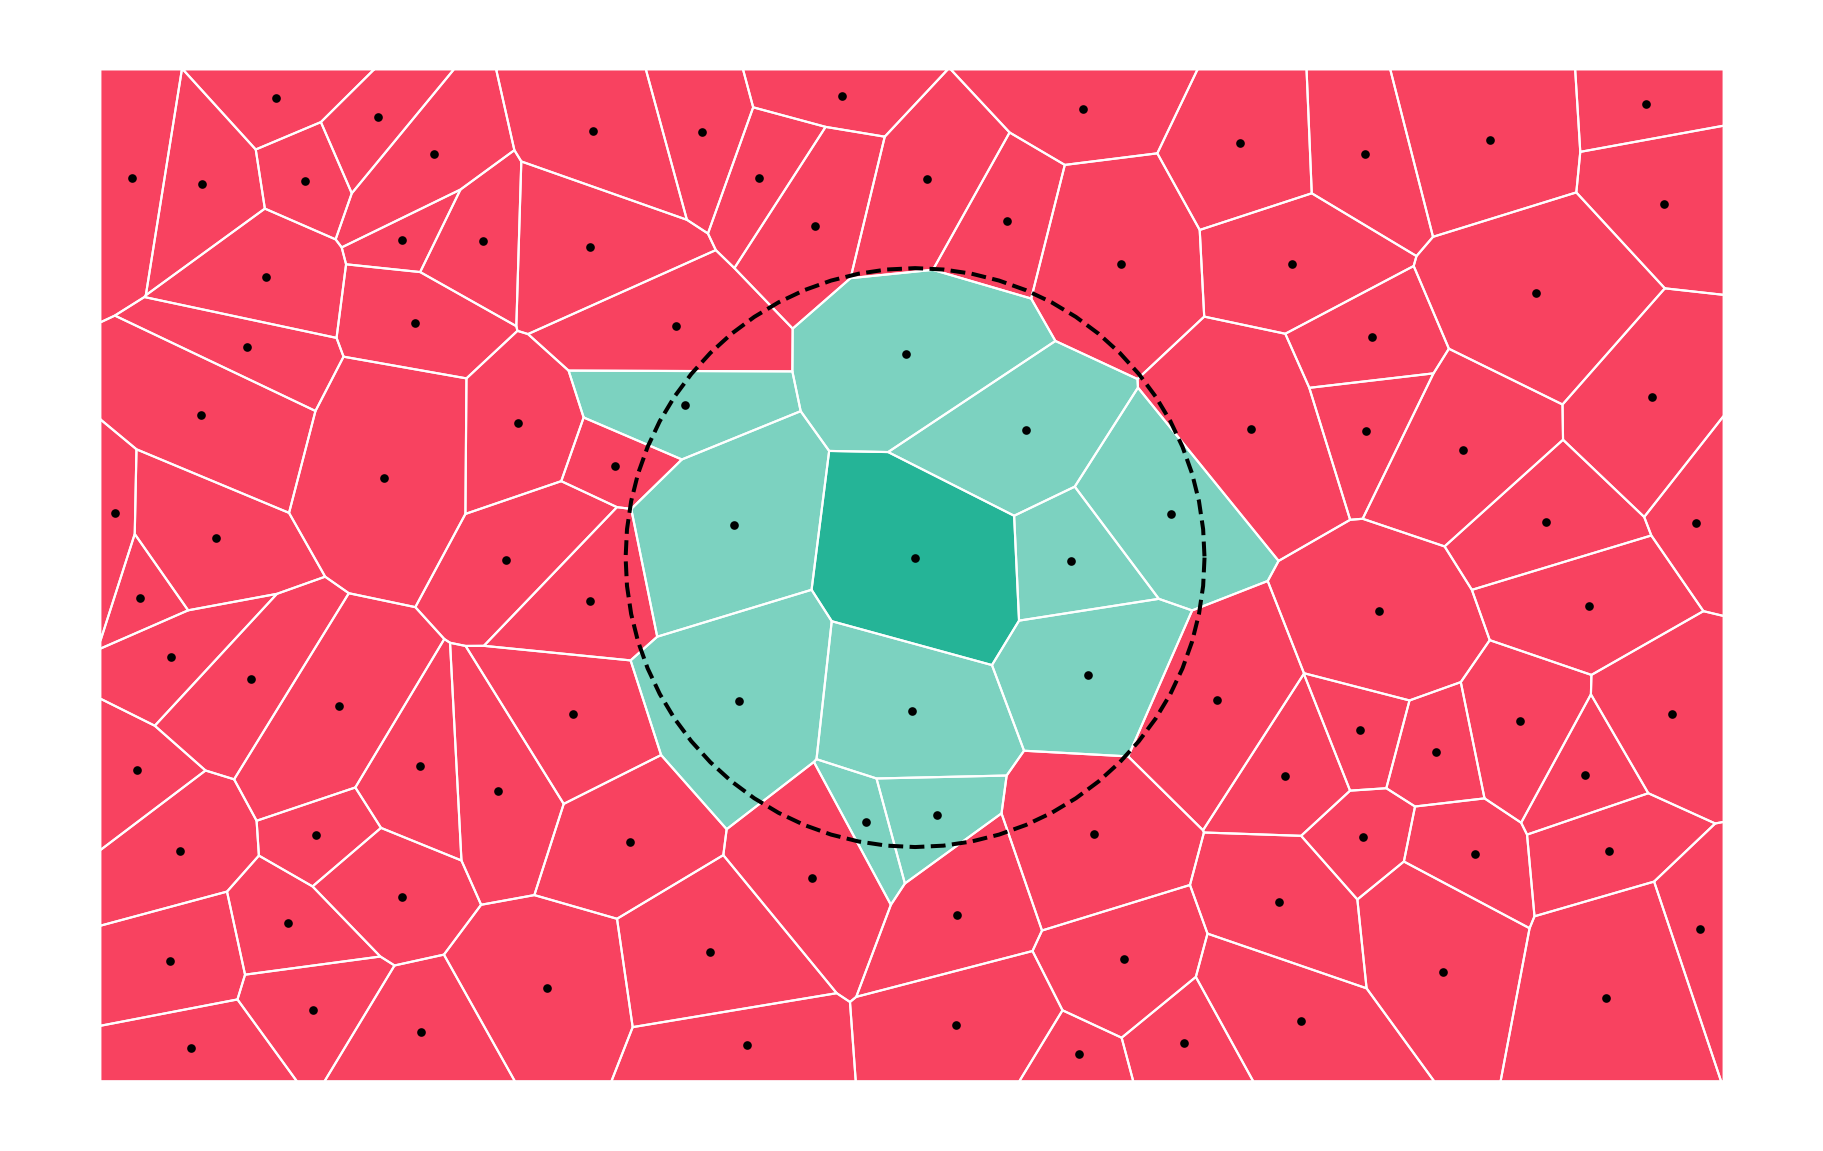
\includegraphics[width=1\linewidth,height=\textheight,keepaspectratio]{images/06-neighbour.png}
\end{center}

Из курса М. Фляйшманна ``Spatial Data Science for Social Geography''
\end{frame}

\begin{frame}{Пространственная автокорреляция}
\phantomsection\label{ux43fux440ux43eux441ux442ux440ux430ux43dux441ux442ux432ux435ux43dux43dux430ux44f-ux430ux432ux442ux43eux43aux43eux440ux440ux435ux43bux44fux446ux438ux44f}
Степень в какой сходные значения находятся рядом.

\begin{itemize}
\tightlist
\item
  положительная автокорреляция: похожие значения находятся рядом
\item
  отрицательная автокорреляция: похожие значения находятся далеко друг
  от друга
\end{itemize}

\pause

\begin{itemize}
\tightlist
\item
  глобальная: имеют ли значения тенденцию оказываться рядом с другими
  похожими/непохожими значениями;
\item
  локальная: существует ли некоторая специфический фрагментм
  пространства, где наблюдается необычная концентрация
  похожими/непохожих значений.
\end{itemize}
\end{frame}

\begin{frame}{Значение Moran I: 0.4763736}
\phantomsection\label{ux437ux43dux430ux447ux435ux43dux438ux435-moran-i-0.4763736}
\pandocbounded{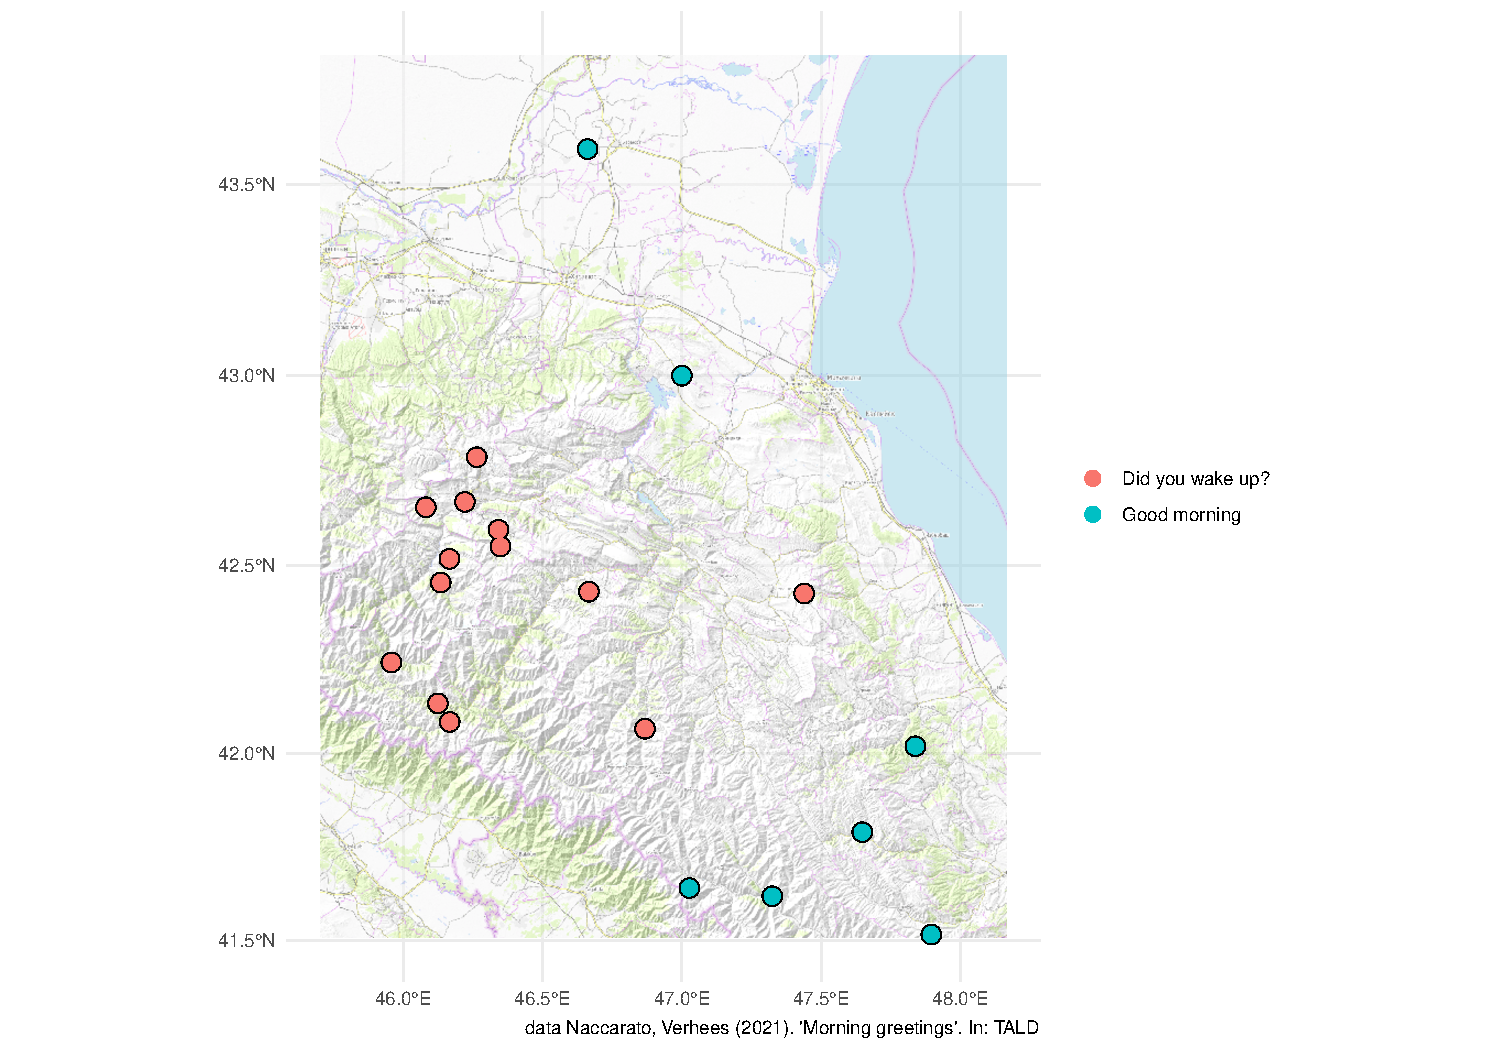
\includegraphics[keepaspectratio]{2025.04.24_HSE_DH_geo_time_files/figure-beamer/unnamed-chunk-19-1.pdf}}
\end{frame}

\begin{frame}{Значение Moran I: -0.1480726}
\phantomsection\label{ux437ux43dux430ux447ux435ux43dux438ux435-moran-i--0.1480726}
\pandocbounded{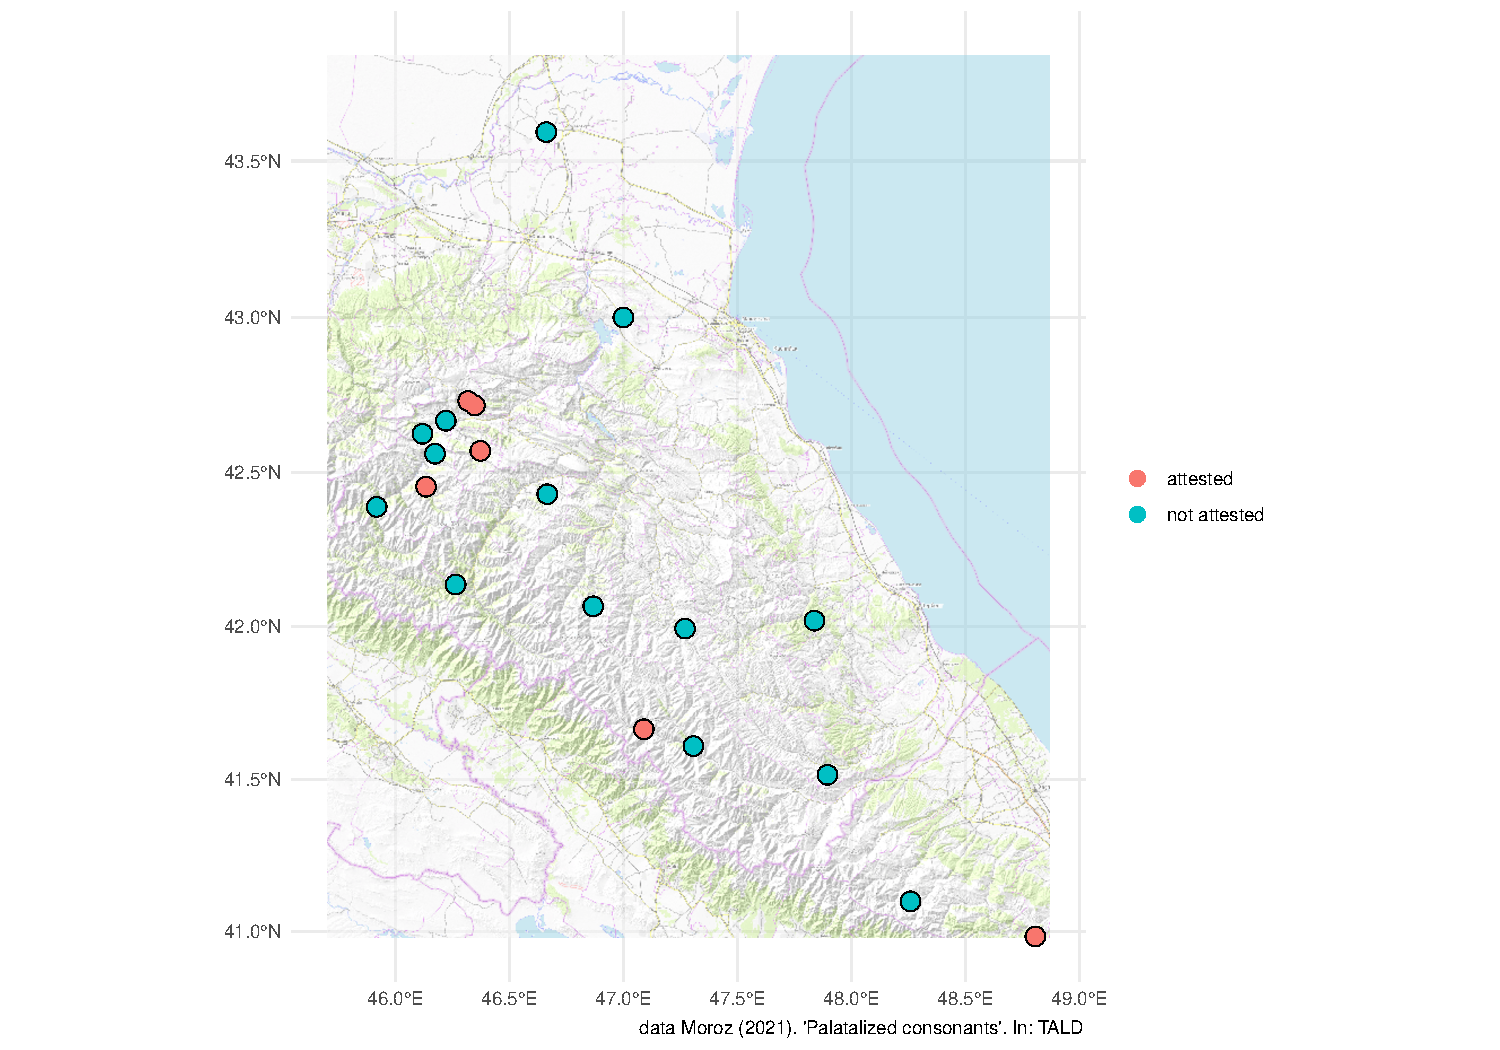
\includegraphics[keepaspectratio]{2025.04.24_HSE_DH_geo_time_files/figure-beamer/unnamed-chunk-22-1.pdf}}
\end{frame}

\begin{frame}{}
\phantomsection\label{section}
Мне хочется выразить благодарность Евгению~Николаевичу~Матерову за его
блог и телеграм-канал ``Наука и
данные''~(\url{https://t.me/naukaidannye}), которые значительно
упростили написание этой лекции, в частности за ссылку на курс Мартина
Фляйшманна ``Spatial Data Science for Social Geography''.
\end{frame}

\section{Временные
данные}\label{ux432ux440ux435ux43cux435ux43dux43dux44bux435-ux434ux430ux43dux43dux44bux435}

\begin{frame}{Переменные бывают разные}
\phantomsection\label{ux43fux435ux440ux435ux43cux435ux43dux43dux44bux435-ux431ux44bux432ux430ux44eux442-ux440ux430ux437ux43dux44bux435}
\begin{center}
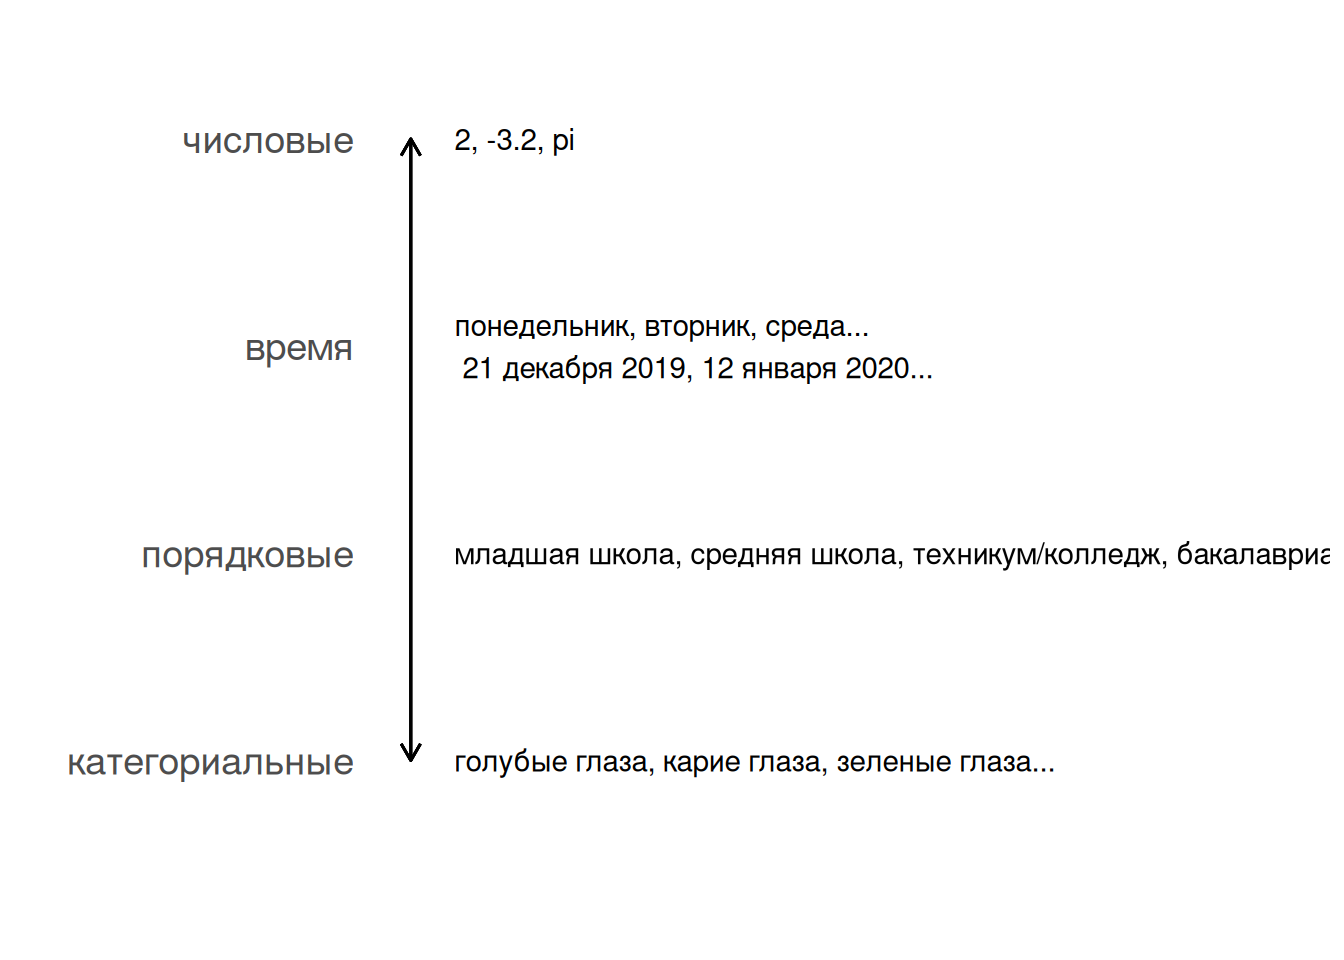
\includegraphics[width=1.08\linewidth,height=\textheight,keepaspectratio]{images/09_time_variable.png}
\end{center}
\end{frame}

\begin{frame}{Переменные бывают разные}
\phantomsection\label{ux43fux435ux440ux435ux43cux435ux43dux43dux44bux435-ux431ux44bux432ux430ux44eux442-ux440ux430ux437ux43dux44bux435-1}
Кажется, что время --- просто обычная числовая переменная, на которой
определены все обычные операции сложения вычитания и т. п. Однако стоит
держать в голове несколько фактов:

\begin{itemize}
\tightlist
\item
  Не каждый год содержит 365 дней. Существуют високосные года. \pause
\item
  Не каждый день содержит 24 часа. Во многих странах используют переход
  на летнее и зимнее время. \pause
\item
  Не в каждой минуте 60 секунд. Существуют дополнительная секунда,
  которую добавляют чтобы компенсировать замедление во вращении земли
  (тогда после секунды 23:59:59 идет секунда 23:59:60). \pause
\item
  Григорианский календарь --- не единственный календарь на свете.
\end{itemize}
\end{frame}




\end{document}
